\documentclass{article}

% Language setting
% Replace `english' with e.g. `spanish' to change the document language
\usepackage[english]{babel}
\usepackage{CJKutf8}
\usepackage{listings}
\usepackage{minted}
% Remove this draft watermark for the final version
% \usepackage{draftwatermark}

% Set page size and margins
% Replace `letterpaper' with `a4paper' for UK/EU standard size
\usepackage[letterpaper,top=2cm,bottom=2cm,left=3cm,right=3cm,marginparwidth=1.75cm]{geometry}

% Useful packages
\usepackage{amsmath}
\usepackage{comment}
\usepackage{graphicx}
\usepackage{IEEEtrantools}
\usepackage[hyphens]{url}
\usepackage[colorlinks=true, allcolors=blue]{hyperref}


\begin{CJK}{UTF8}{min}
\title{Aptosブロックチェーン:安全、スケーラブル、アップグレード可能なWeb3インフラ}
\author{}
\date{2022年8月11日\\v1.0}

\begin{document}
\maketitle

\renewcommand{\abstractname}{要約}
\renewcommand{\figurename}{絵}

\begin{CJK}{UTF8}{min}
新しいインターネットインフラとしてのブロックチェーンの台頭により、開発者は何万もの分散型アプリケーションを急速にデプロイしています。残念ながら、ブロックチェーンの利用は、頻繁な停止、高いコスト、低いスループット制限、および多くのセキュリティ上の懸念のために、まだユビキタスではありません。Web3時代に大量導入を可能にするためには、ブロックチェーンインフラは、広く利用されるアプリケーションを構築するための信頼性の高い、拡張性の高い、コスト効率の良い、継続的に改善されるプラットフォームとして、クラウドインフラの道を歩む必要があります。

これらの課題を解決するために、スケーラビリティ、安全性、信頼性、アップグレード可能性を重要な原則として設計された \emph{Aptos ブロックチェーン}を発表します。Aptosブロックチェーンは、世界中の350人以上の開発者によって、過去3年間にわたり開発されてきました。\cite{aptos_core_github}. Aコンセンサス、スマートコントラクト設計、システムセキュリティ、パフォーマンス、および分散化において、新しく斬新なイノベーションを提供しています。これらの技術の組み合わせは、web3を大衆に届けるための基本的なビルディングブロックを提供します。:\footnote{法的免責事項:本ホワイトペーパーとその内容は、トークンの販売や購入の申し出の勧誘を目的としたものではありません。私たちは、一般の方々からフィードバックやコメントをいただくためにのみ、このホワイトペーパーを発行しています。この文書のいかなる部分も、Aptosブロックチェーンまたはそのトークン(もしあれば)がどのように発展し、利用され、または価値を生むかを保証または約束するものとして読んだり解釈してはなりません。Aptosは現在の計画を概説しているだけであり、その計画は同社の裁量で変更可能であり、その成功は同社の管理外の多くの要因に依存します。このような将来の記述は、必然的に既知および未知のリスクを伴い、将来の期間における実際のパフォーマンスや結果は、このホワイトペーパーで説明または暗示したものと大きく異なる可能性があります。Aptosは、計画を更新する義務を負いません。実際の結果や将来の出来事が大きく異なる可能性があるため、ホワイトペーパーのいかなる記述も正確であることを保証するものではありません。将来の記述に過度の信頼を置かないようにお願いします。}
 
 \begin{itemize}
  \item まず、Aptosブロックチェーンは 、 \emph{Move言語}をネイティブに統合し、内部で使用して、高速で安全なトランザクションを実行します\cite{move_github}。Move言語で記述されたスマートコントラクトのための正式な検証機である \emph{Move prover} は、コントラクトの不変量と動作にさらなる安全策を提供します。このようにセキュリティを重視することで、開発者は自分たちのソフトウェアを悪意ある存在からよりよく保護することができます。開発者は、悪意のあるエンティティからソフトウェアをよりよく保護することができます。
  
  \item 第二に、Aptosのデータモデルは、柔軟なキー管理とハイブリッドカストディアルオプションを可能にします。これは、署名前のトランザクションの透明性と実用的な軽量クライアントプロトコルと共に、より安全で信頼できるユーザーエクスペリエンスを提供します。
  
  \item 第三に、高いスループットと低レイテンシーを実現するために、Aptosブロックチェーンはトランザクション処理の主要段階において、パイプライン化されたモジュール式のアプローチを活用しています。具体的には、取引の普及、ブロックメタデータの順序付け、並列取引の実行、バッチストレージ、元帳の認証のすべてが同時に動作します。このアプローチにより、利用可能なすべての物理リソースをフルに活用し、ハードウェア効率を向上させ、高度な並列実行を可能にします。
  
  \item 第四に、他の並列実行エンジンでは、読み書きの対象となるデータについて前もって知る必要があるため、トランザクションの原子性が壊れてしまいますが、Aptosブロックチェーンでは、開発者にそのような制限を設けていません。任意に複雑なトランザクションの原子性を効率的にサポートし、実世界のアプリケーションでより高いスループットと低レイテンシーを実現し、開発を簡素化することが可能です。
  
 \item 第5に、Aptosのモジュラーアーキテクチャ設計は、クライアントの柔軟性をサポートし、頻繁かつ即時のアップグレードに最適化されています。さらに、新しい技術革新を迅速に展開し、新しいWeb3のユースケースをサポートするために、Aptosブロックチェーンは、組み込みのオンチェーン変更管理プロトコルを提供します。
 
 \item 最後に、Aptosブロックチェーンは、個々のバリデータの性能を超えるスケールアップのための将来のイニシアチブを実験しています。そのモジュール設計と並列実行エンジンはバリデータの内部シャーディングをサポートし、同種の状態シャーディングは、ノードオペレータに複雑さを追加することなく水平方向のスループット拡張性の可能性を提供します。
\end{itemize}

\end{CJK}

\section{はじめに}
\label{sec:introduction}

Web2版インターネットでは、メッセージング、ソーシャルメディア、金融、ゲーム、ショッピング、オーディオ/ビデオストリーミングなどのサービスが、ユーザーデータへの直接アクセスを制御する中央集権的企業(Google、Amazon、Apple、Metaなど)によって提供されています。これらの企業は、対象となるユースケースに最適化されたアプリケーション固有のソフトウェアを使用してインフラを開発し、クラウドインフラストラクチャを活用してこれらのアプリケーションをユーザーに展開します。クラウドインフラは、世界中のデータセンター(例:AWS、Azure、Google Cloud)で稼働するレンタル仮想マシン(VM)やベアメタルハードウェアなど、仮想化・物理化されたインフラサービスへのアクセスを提供します。その結果、何十億人ものユーザーに対応できるweb2インターネットサービスの構築が、今日ほど容易になったことはありません。しかし、web2では、ユーザーが中央集権的なエンティティに明示的な信頼を置く必要があり、この要件は社会的にますます懸念されるようになってきています。

この懸念に対抗するため、新しいインターネットの時代、web3が始まりました:web3では\emph{ブロックチェーン} が登場し、分散化された不変の台帳を提供することで、ユーザー同士が安全かつ確実にやりとりできるようになり、仲介者や中央集権的なエンティティを信頼する必要がありません。Web2インターネットサービスやアプリケーションがビルディングブロックとしてクラウドインフラに依存しているのと同様に、分散型アプリケーションはブロックチェーンを分散型インフラ層として利用し、世界中の何十億ものユーザーにリーチすることができます。

しかし、今日、多くのブロックチェーンが存在するにもかかわらず、web3の広範な採用はまだ行われていません~\cite{a16_state}。 テクノロジーは業界を進歩させ続けていますが、既存のブロックチェーンは信頼性が低く、ユーザーに高い取引手数料を課し、スループットの制限が低く、セキュリティ問題による定期的な資産損失に苦しみ、リアルタイムの応答性をサポートすることができないのです。クラウドインフラがWeb2サービスを数十億人に届けることを可能にしたのに比べ、ブロックチェーンはWeb3アプリケーションを同じように実現するには至っていません。

\section{Aptosのビジョン}
\label{sec:aptos_vision}

Aptosのビジョンは、Web3に主流をもたらし、実世界のユーザーの問題を解決する分散型アプリケーションのエコシステムを強化することができるブロックチェーンを提供することです。私たちの使命は、柔軟でモジュール化されたブロックチェーンアーキテクチャを提供することにより、ブロックチェーンの信頼性、安全性、性能における最先端を前進させることです。このアーキテクチャは、頻繁なアップグレード、最新の技術の進歩の迅速な採用、新しいユースケースや新興のユースケースに対するファーストクラスのサポートをする必要があります。

私たちは、分散型で安全かつスケーラブルなネットワークが、それを利用するコミュニティによって管理・運営されることを想定しています。世界中でインフラの需要が高まれば、ブロックチェーンの計算資源は水平方向にも垂直方向にもスケールアップして、そのニーズに応えます。新しいユースケースや技術的な進歩が生じると、ネットワークはユーザーを中断させることなく、頻繁にシームレスにアップグレードされるはずです。そしてインフラに関する懸念も、背景に薄れていくはずです。開発者とユーザーは、キーの復元、データモデリング、スマートコントラクトの標準、リソース使用のトレードオフ、プライバシー、およびコンポーザビリティに関する多くの異なるオプションにアクセスすることができます。ユーザーは、自分の資産が安全で、常に利用可能であり、ほぼ原価(低料金)でアクセスできることを知ることができます。そして、誰もが安全、簡単、かつ不変に世界中の信頼できない相手と取引することができます。ブロックチェーンは、クラウドインフラと同じようにユビキタスな存在です。

このビジョンを達成するためには、大幅な技術的進歩を遂げる必要があります。過去3年間にわたるDiemブロックチェーン(Aptosブロックチェーンの前身)の構築、開発、進歩、展開の経験から、ネットワークはクライアントを混乱させることなくプロトコルを継続的にアップグレードできることが証明されています~\cite{diem_blockchain}。Diemメインネットは、2020年初頭に複数のウォレットプロバイダーとともに10数社のノードオペレーターに展開されました。その後の1年間で、私たちのチームはコンセンサスプロトコルとコアフレームワークを変更する2つのメジャーアップグレードを発行しました。どちらのアップグレードも、ユーザーにダウンタイムを与えることなく完了しました。Aptosブロックチェーンでは、Diemブロックチェーンに触発され、安全かつ透明で頻繁なアップグレードを中核機能として取り入れながら、技術スタックに一連の抜本的な改良を施したのです。特に、(セクション7で説明する\ref{sec:pipelining_batching}) トランザクション処理の斬新な手法と、分散化とネットワークガバナンスへの新たなアプローチを強調しています。

Aptosブロックチェーンが改善され成長し続けるにつれ、私たちはこのホワイトペーパーの最新版を発行し、私たちのプロトコルと設計の選択を更新していく予定です。この文書の残りの部分では、Aptosブロックチェーンの現在の状態と将来の計画について説明します。

\begin{figure}
\centering
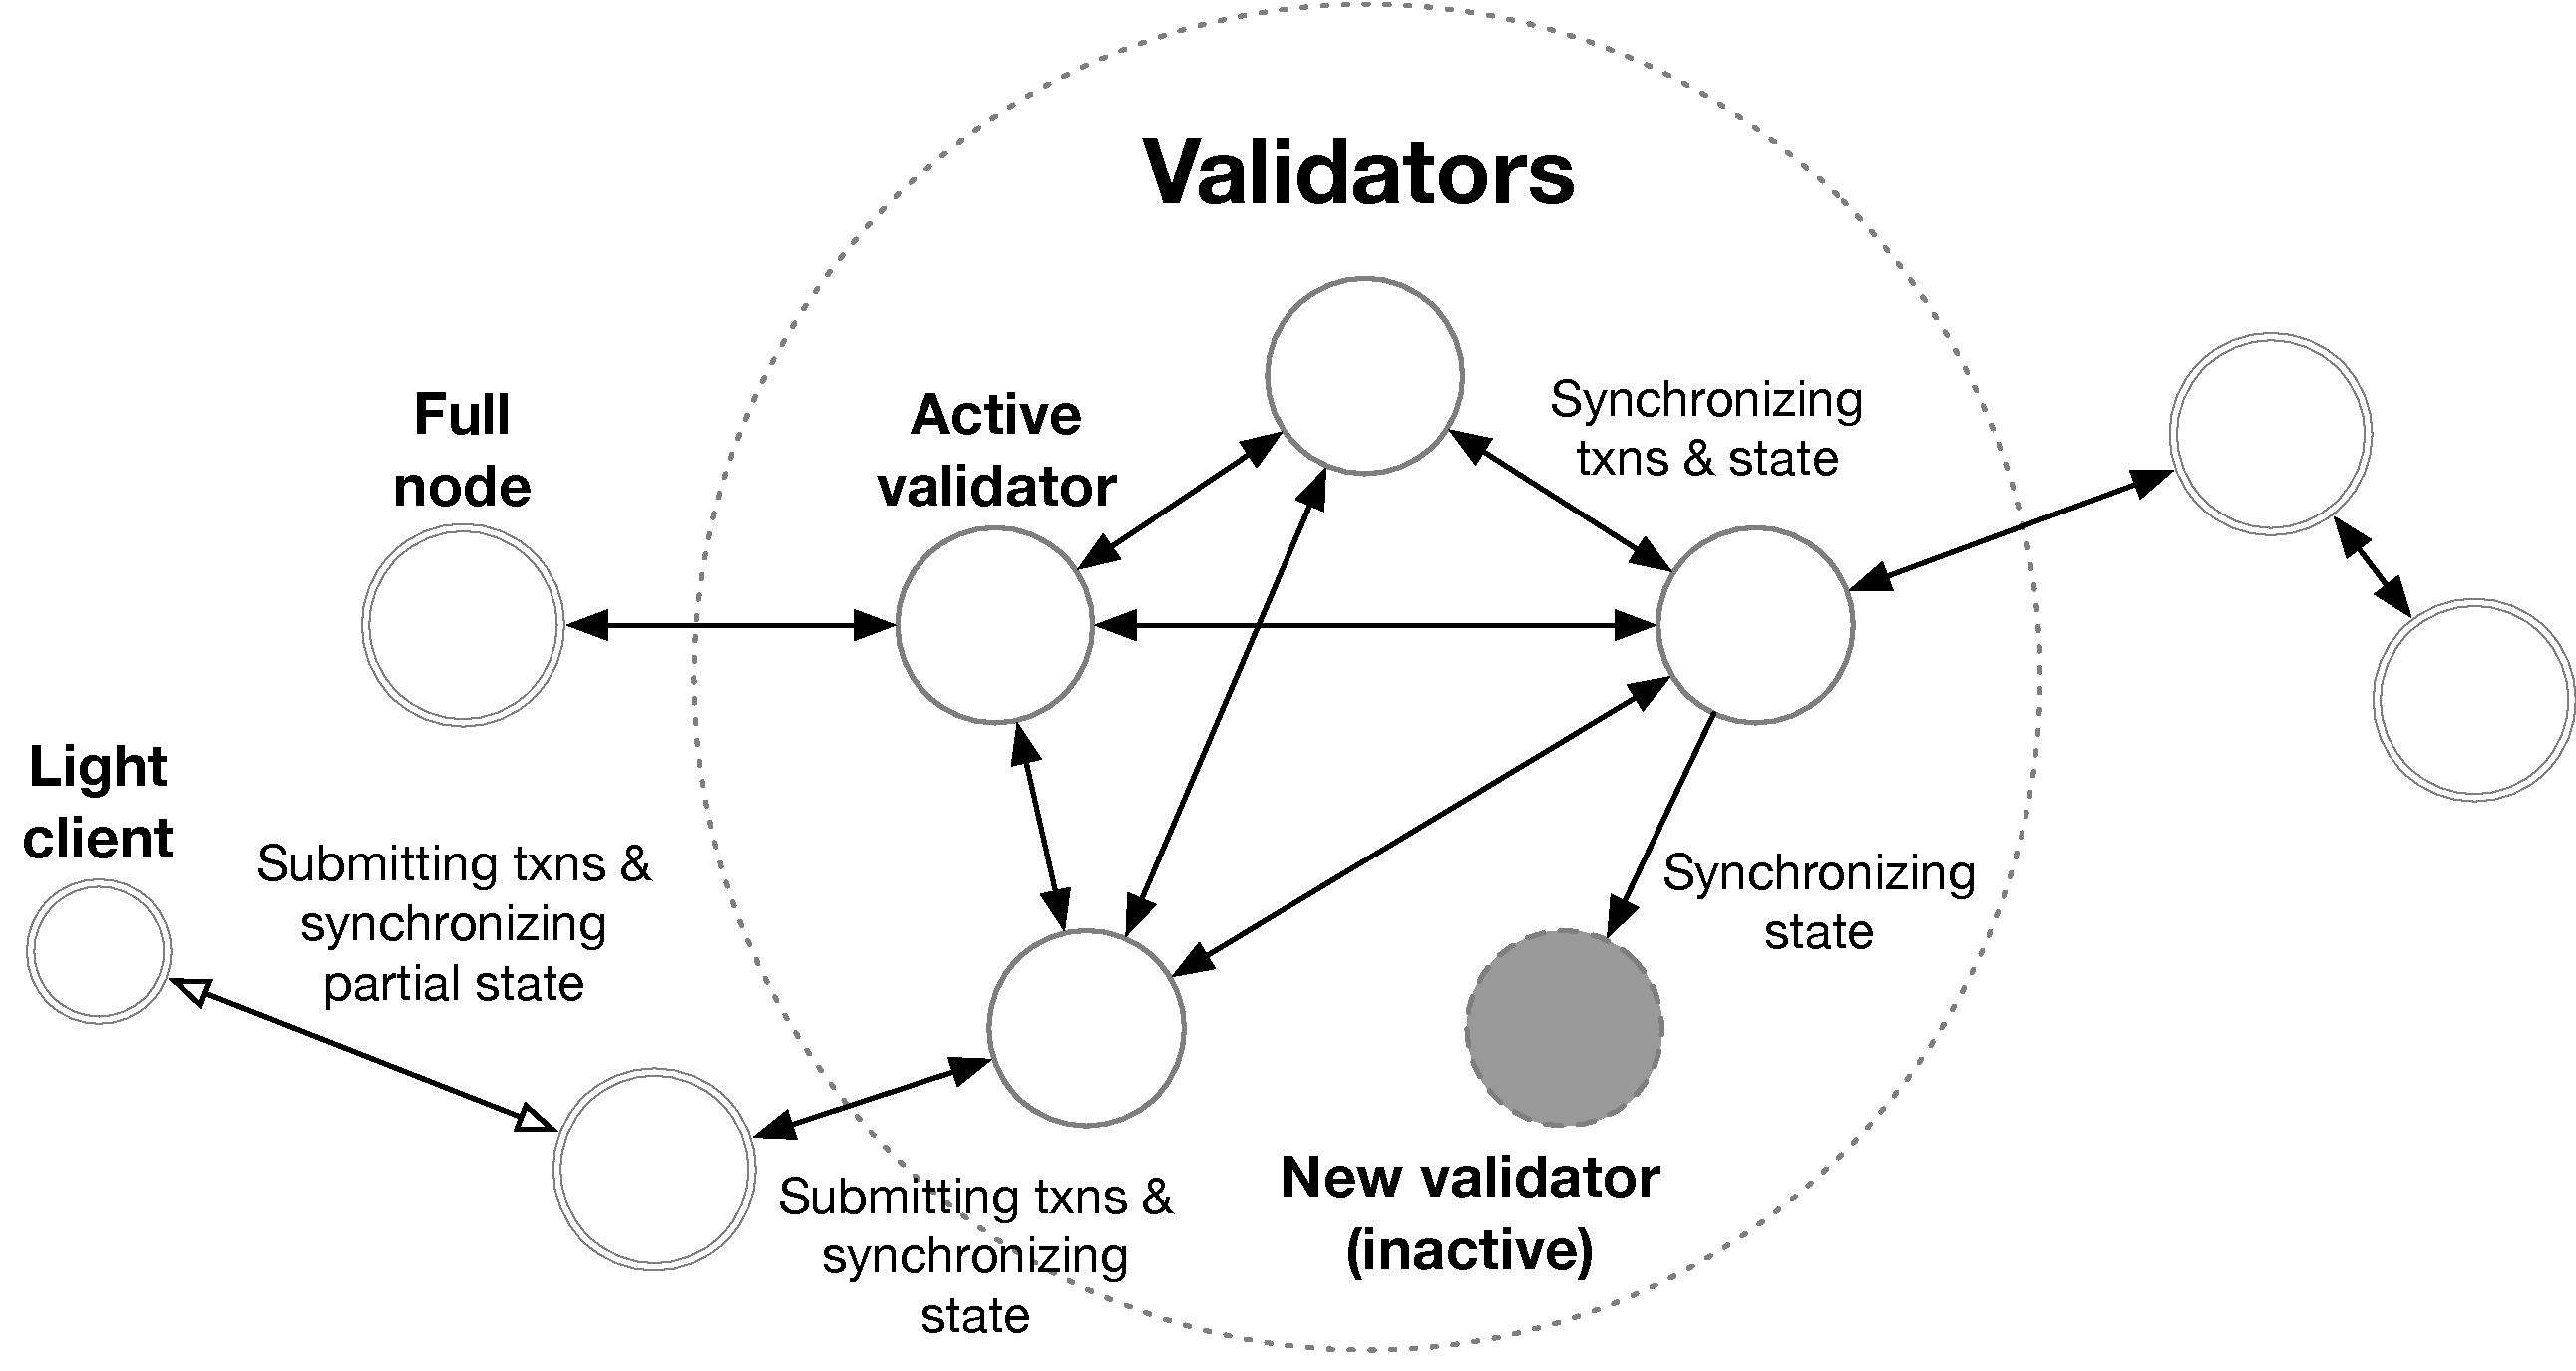
\includegraphics[width=0.9\textwidth]{validators.pdf}
\caption{\label{fig:aptos_ecosystem}Aptosエコシステムの構成要素}
\end{figure}

\section{概要}
\label{sec:overview}

Aptosブロックチェーンは、図~\ref{fig:aptos_ecosystem}に示すように、 byzantineフォールトトレラント (\emph{BFT})、プルーフオブステーク合意メカニズムを使用してユーザーからの取引を共同で受信し処理する\emph{バリデーター} のセットで構成されています。トークン保有者は、選択したバリデーターにトークンを \emph{ステーク} し、ロックします。各バリデーターのコンセンサス投票の比重は、そのバリデーションに賭けられた金額に比例します。バリデータは\emph{アクティブ} であり、コンセンサスに参加することができます。同様に、バリデータは、参加するのに十分なステークがない場合、バリデータセットから外れる場合、 ブロックチェーンの状態を同期するためにオフラインになる場合、あるいは過去のパフォーマンスが 低いためにコンセンサスプロトコルから不参加とみなされた場合、\emph{ 非アクティブ} になることがあります。 クライアントとは、取引を提出したり、ブロックチェーンの状態や履歴を照会したりする必要があるシステムのあらゆる部分を指します

\emph{クライアント} は、照会されたデータのバリデータ署名付き証明をダウンロードし、検証することを選択できます。
\emph{フルノード} は、バリデータまたはネットワーク上の他のフルノードから取引とブロックチェーンの 状態を複製するクライアントです。また、必要に応じて取引履歴やブロックチェーンの状態を削除し、ストレージを再利用することも可能です。
\emph{ライトクライアント} は現在のバリデータのみを保持し、部分的なブロックチェーンの状態を、通常フルノードから安全に問い合わせることができます。ウォレットはライトクライアントの一般的な例です。 安全、高速、信頼性が高く、アップグレード可能なWeb3インフラの普及のニーズを満たすため、Aptosブロックチェーンは以下のコア設計原則に基づいて構築されています。

安全、高速、信頼性が高く、アップグレード可能なWeb3インフラの普及のニーズを満たすため、Aptosブロックチェーンは以下のコア設計原則に基づいて構築されています。

\begin{itemize}
 \item 新しいスマートコントラクトプログラミング言語Move \cite{move}を介して、高速で安全な実行と簡単な監査可能性、機械的な分析可能性を実現します。 Aptosブロックチェーンの前身から始まり、このプロジェクトの進化とともに進歩し続けています。
 
 \item バッチ処理、パイプライン処理、並列処理によるトランザクション処理で、極めて高いスループットと低レイテンシーを実現します。
 
 \item 読み書きの対象となるデータ位置を前もって知る必要がある既存の並列実行エンジンとは異なり、Block-STMによって任意に複雑なトランザクションの原子性を効率的にサポートする新規な並列トランザクション処理します。
 
 \item 迅速なステークウェイトバリデータセットのローテーションとレピュテーショントラッキングにより、パフォーマンスと分散化のための最適化を実現します。
 
 \item 新しいユースケースと最新技術を受け入れるための第一級の設計原則としてのアップグレード性とコンフィギュラビリティ。
 
 \item モジュール設計により、コンポーネントレベルでの厳格なテスト、適切な脅威のモデル化、シームレスな展開を実現し、高い安全性と信頼性のある運用を保証します。
 
 \item シャーディングは、ユーザーに公開され、プログラミングとデータモデルにネイティブなファーストクラスのコンセプトであるため、分散化を維持したまま水平方向のスループット拡張が可能です。
 
\end{itemize}
セクション\ref{sec:move}開発者がAptosブロックチェーンのMoveとどのようにやり取りするかを説明します。セクション\ref{sec:logical}では、論理データモデルについて説明します。セクション \ref{sec:user}では、Aptosブロックチェーンが強力な検証方法を通じて安全なユーザーエクスペリエンスを可能にする方法を詳しく説明します。セクション\ref{sec:pipelining_batching}では、パイプライン、バッチ処理、並列化に関する主要なパフォーマンス革新について説明します。セクション\ref{sub:state_sync}では、異なるクライアントが他のノードと状態を同期させるための様々なオプションについて詳しく説明します。セクション\ref{sec:community_ownership}は、コミュニティのオーナーシップとガバナンスのための計画について説明します。最後に、セクション10では、分散化を維持しつつ、将来の性能の方向性について議論します。

\section{Move言語}
\label{sec:move}

Moveは、安全性と柔軟性に重点を置いた新しいスマートコントラクトプログラミング言語です。Aptosブロックチェーンは、Moveのオブジェクトモデルを使用して台帳の状態を表現し(セクション\ref{sub:ledger_state}参照)、Moveコード(モジュール)を使用してステートトランザクションのルールを符号化します。ユーザーは、新しいモジュールの公開、既存のモジュールのアップグレード、モジュール内で定義されたエントリ関数の実行、またはモジュールのパブリックインターフェースと直接対話できるスクリプトを含むトランザクションを提出します

Moveのエコシステムには、コンパイラー、仮想マシン、その他多くの開発者向けツールが含まれます。Moveはプログラミング言語Rustにインスパイアされており、線形型のような概念によってデータの所有権を言語内で明示することができます。Moveはリソースの希少性、保存性、アクセス制御を重視しています。Moveのモジュールは、すべてのリソースの寿命、保存、アクセスパターンを定義しています。これにより、 \mintinline{rust}{コイン}のようなリソースが適切な認証情報なしに生成されたり、二重に消費されたり、消滅したりすることがないようにします。

Moveはバイトコード検証器を活用し、信頼されていないコードが存在する場合でも、型とメモリの安全性を保証します。より信頼できるコードを書くために、Moveには形式検証器Move Prover\cite{move_prover}があり、Moveに統合された仕様言語で定式化された仕様に対してMoveプログラムの機能が正しいかどうかを検証することができます。

ユーザーアカウントと対応するアカウントコンテンツに加え、台帳の状態にはAptosブロックチェーンのオンチェーン構成も含まれます。このネットワーク構成には、アクティブなバリデータのセット、ステーキングプロパティ、およびAptosブロックチェーン内のさまざまなサービスの構成が含まれます。Moveのモジュールアップグレード可能性と包括的なプログラム可能性のサポートは、シームレスな構成変更を可能にし、Aptosブロックチェーン自体のアップグレードをサポートします(アップグレードの両方のセットは、プライベートメインネット上でゼロダウンタイムで複数回実行されています)。

Aptosチームは、より広範なWeb3のユースケースをサポートすることで、Moveをさらに強化しました。セクション\ref{sub:ledger_state}で後述するように、Aptosブロックチェーンはきめ細かなリソース制御を可能にします。これは実行の並列化をサポートするだけでなく、データへのアクセスや変異に関連するほぼ固定されたコストを実現します。さらに、Aptosブロックチェーンは、きめ細かいストレージの上に構築されたテーブルサポートを提供し、単一のアカウントで大規模なデータセット(例えば、NFTの大規模なコレクション)を使用できるようにします。さらに、Aptosは、完全にオンチェーンで表現される共有または自律アカウントに対応しています。これにより、複雑な分散型自律組織(DAO)が共同でアカウントを共有したり、これらのアカウントをリソースの異種コレクションのコンテナとして使用したりすることができます。

\section{論理データモデル}
\label{sec:logical}

Aptosブロックチェーンの\emph{l元帳の状態}は、すべてのアカウントの状態を表します。台帳の状態は、システムが実行した取引数に対応する符号なし64ビット整数を使用してバージョン管理されています。誰でもAptosブロックチェーンにトランザクションを提出し、元帳の状態を変更することができます。トランザクションが実行されると、 \emph{トランザクション出力}が生成されます。トランザクション出力は、台帳の状態を操作するゼロ以上の操作( \emph{書き込みセット}と呼ばれる)、結果イベントのベクトル(セクショ ン \ref{subsub:events}参照)、消費されたガスの量、および実行されたトランザクションの状態を含んでいます。

\subsection{トランザクション}

署名されたトランザクションは、以下の情報を含みます。

\begin{itemize}
 \item \textbf{トランザクション認証機能}:送信者は、トランザクションが認証されたことを確認するために、1つまたは複数のデジタル署名を含むトランザクション認証機能を使用します。
 
 \item \textbf{送信者アドレス}:送信者のアカウントアドレス。
 
 \item \textbf{ペイロード}:ペイロードは、チェーン上の既存のエントリ関数を参照するか、インライン バイトコードとして実行される関数を含みます(スクリプトと呼ばれます)。さらに、入力引数のセットはバイト配列でエンコードされます。peer-to-peer取引の場合、入力には受取人の情報とその受取人に送金される金額が含まれます。
 
 \item \textbf{ガス価格}(指定通貨/ガス単位):取引実行のために、送り手がガス1単位あたり支払う金額です。ガスとは、計算機、ネットワーク、ストレージの代金を支払う方法です。ガス単位は計算の抽象的な測定値であり、現実世界での固有の価値はありません。

 \item \textbf{最大ガス量}:最大ガス量は、トランザクションが中断される前に消費することが許される最大ガス単位です。アカウントは少なくともガス価格に最大ガス量を掛けたものを持っていなければならず、さもなければ検証中にトランザクションが破棄されます。
 
 \item \textbf{Sequence番号}:トランザクションのSequence番号です。これは、取引実行時に送信者のアカウントに保存されているSequence番号と一致しなければなりません。トランザクションが正常に実行されると、リプレイ攻撃を防ぐためにアカウントのSequence番号がインクリメントされます。

 \item \textbf{有効期限}:トランザクションが有効でなくなるまでのタイムスタンプです。

 \item \textbf{チェーンID}:このトランザクションが有効なブロックチェーンを特定するもので、署名ミスを防ぐためにユーザーをさらに保護します。

\end{itemize}
各バージョン $i$において、状態変化はタプル $(T_i, O_i, S_i)$で表され、それぞれ取引、取引出力、結果の元帳状態を含みます。決定論的関数 $\textsf{Apply}$が与えられると、元帳状態 $S_{i-1}$ を持つトランザクション $T_i$の実行は、トランザクション出力 $O_i$ と新しい元帳状態 $S_i$を生成します。すなわち、 $\textsf{Apply}(S_{i-1}, T_i) \rightarrow \langle O_i, S_i\rangle$ です。

\subsubsection{イベント}
\label{subsub:events}

イベントはトランザクションの実行中に発行されます。各Moveモジュールは独自のイベントを定義し、実行時にそのイベントを発するタイミングを選択することができます。例えば、コインの送金時には、送り手と受け手の両方のアカウントからそれぞれ \emph{SentEvent}と \emph{ReceivedEvent}が発信されます。このデータは台帳内に保存され、Aptosノード経由で照会することができます。登録されたイベントにはそれぞれ固有のキーがあり、そのキーを使ってイベントの詳細を照会することができます。

同じイベントキーに発行された複数のイベントは、 \emph{イベントストリーム}、0から始まる順次増加する番号、タイプ、およびデータを含む各エントリを持つイベントのリストを生成します。各イベントは、何らかの型によって定義されなければなりません。特にジェネリックを使用している場合、同じまたは類似の型によって定義された複数のイベントが存在する可能性があります。イベントには関連するデータがあります。Moveモジュール開発者にとって一般的な原則は、データを変更しイベントを放出したトランザクションの実行前と実行後の基礎となるリソースの変更を理解するために必要なすべてのデータを含めることです。

トランザクションはイベントを生成することだけが可能で、イベントを読み取ることはできません。この設計により、トランザクションの実行は、履歴情報(例えば、以前に生成されたイベント)ではなく、現在の状態とトランザクションの入力のみの関数であることができます。

\subsection{アカウント}
\label{sec:accounts}

各アカウントは、アカウントアドレスと呼ばれる256ビットの一意の値で識別されます。新しいアカウントは、既存のアカウントから送信されたトランザクションが \mintinline{rust}{create_account(addr)}Move関数を呼び出したときに、元帳状態(セクション \ref{sub:ledger_state}参照)に作成されます。これは通常、トランザクションがまだ作成されていないアカウントアドレスにAptosトークンを送信しようとするときに起こります。利便性のために、Aptosは、転送前にまだ存在しない場合、暗黙的にアカウントを作成する\mintinline{rust}{transfer(from, to, amount)} 関数もサポートしています。

新しいアカウントを作成するために、ユーザはまず署名鍵ペア: $(vk, sk)$を生成します。次に、公開検証鍵 $vk$ の暗号ハッシュ $H$ を署名方式識別子(ssid)と結合して、所定の署名方式の新しいアカウントアドレスを導出します:$(ssid)$: where $addr = H(vk, ssid)$。

アドレス \mintinline{rust}{addr}に新しいアカウントが作成された後、ユーザーはプライベート署名キー $sk$を使って \mintinline{rust}{addr}のアカウントから送信されるトランザクションに署名することができます。またユーザーは、$sk$を積極的に変更するため、または漏洩の可能性に対応するため、$sk$をローテートすることができます。アカウントアドレスは、作成時に公開検証キーから一度だけ導出されるため、これによってアカウントアドレスが変更されることはありません。

Aptosブロックチェーンは、アカウントを実世界のアイデンティティにリンクさせません。ユーザーは複数のキーペアを生成することで複数のアカウントを作成することができます。同じユーザーによって管理されるアカウントは、互いに本質的なつながりを持ちません。しかし、1人のユーザーが複数のアカウントを1つのウォレットで管理し、簡単な資産管理を行うことは可能です。この柔軟性により、将来のリリースに向けてプライバシーを保護するプリミティブを実験している間、ユーザーには仮名性が提供されます。一人のユーザーまたは一組のユーザーによって所有される複数のアカウントは、セクション\ref{subsec:parallel_transaction_execution}で説明するように、実行の並行性を高めるためのチャンネルも提供します。

\begin{figure}
\centering
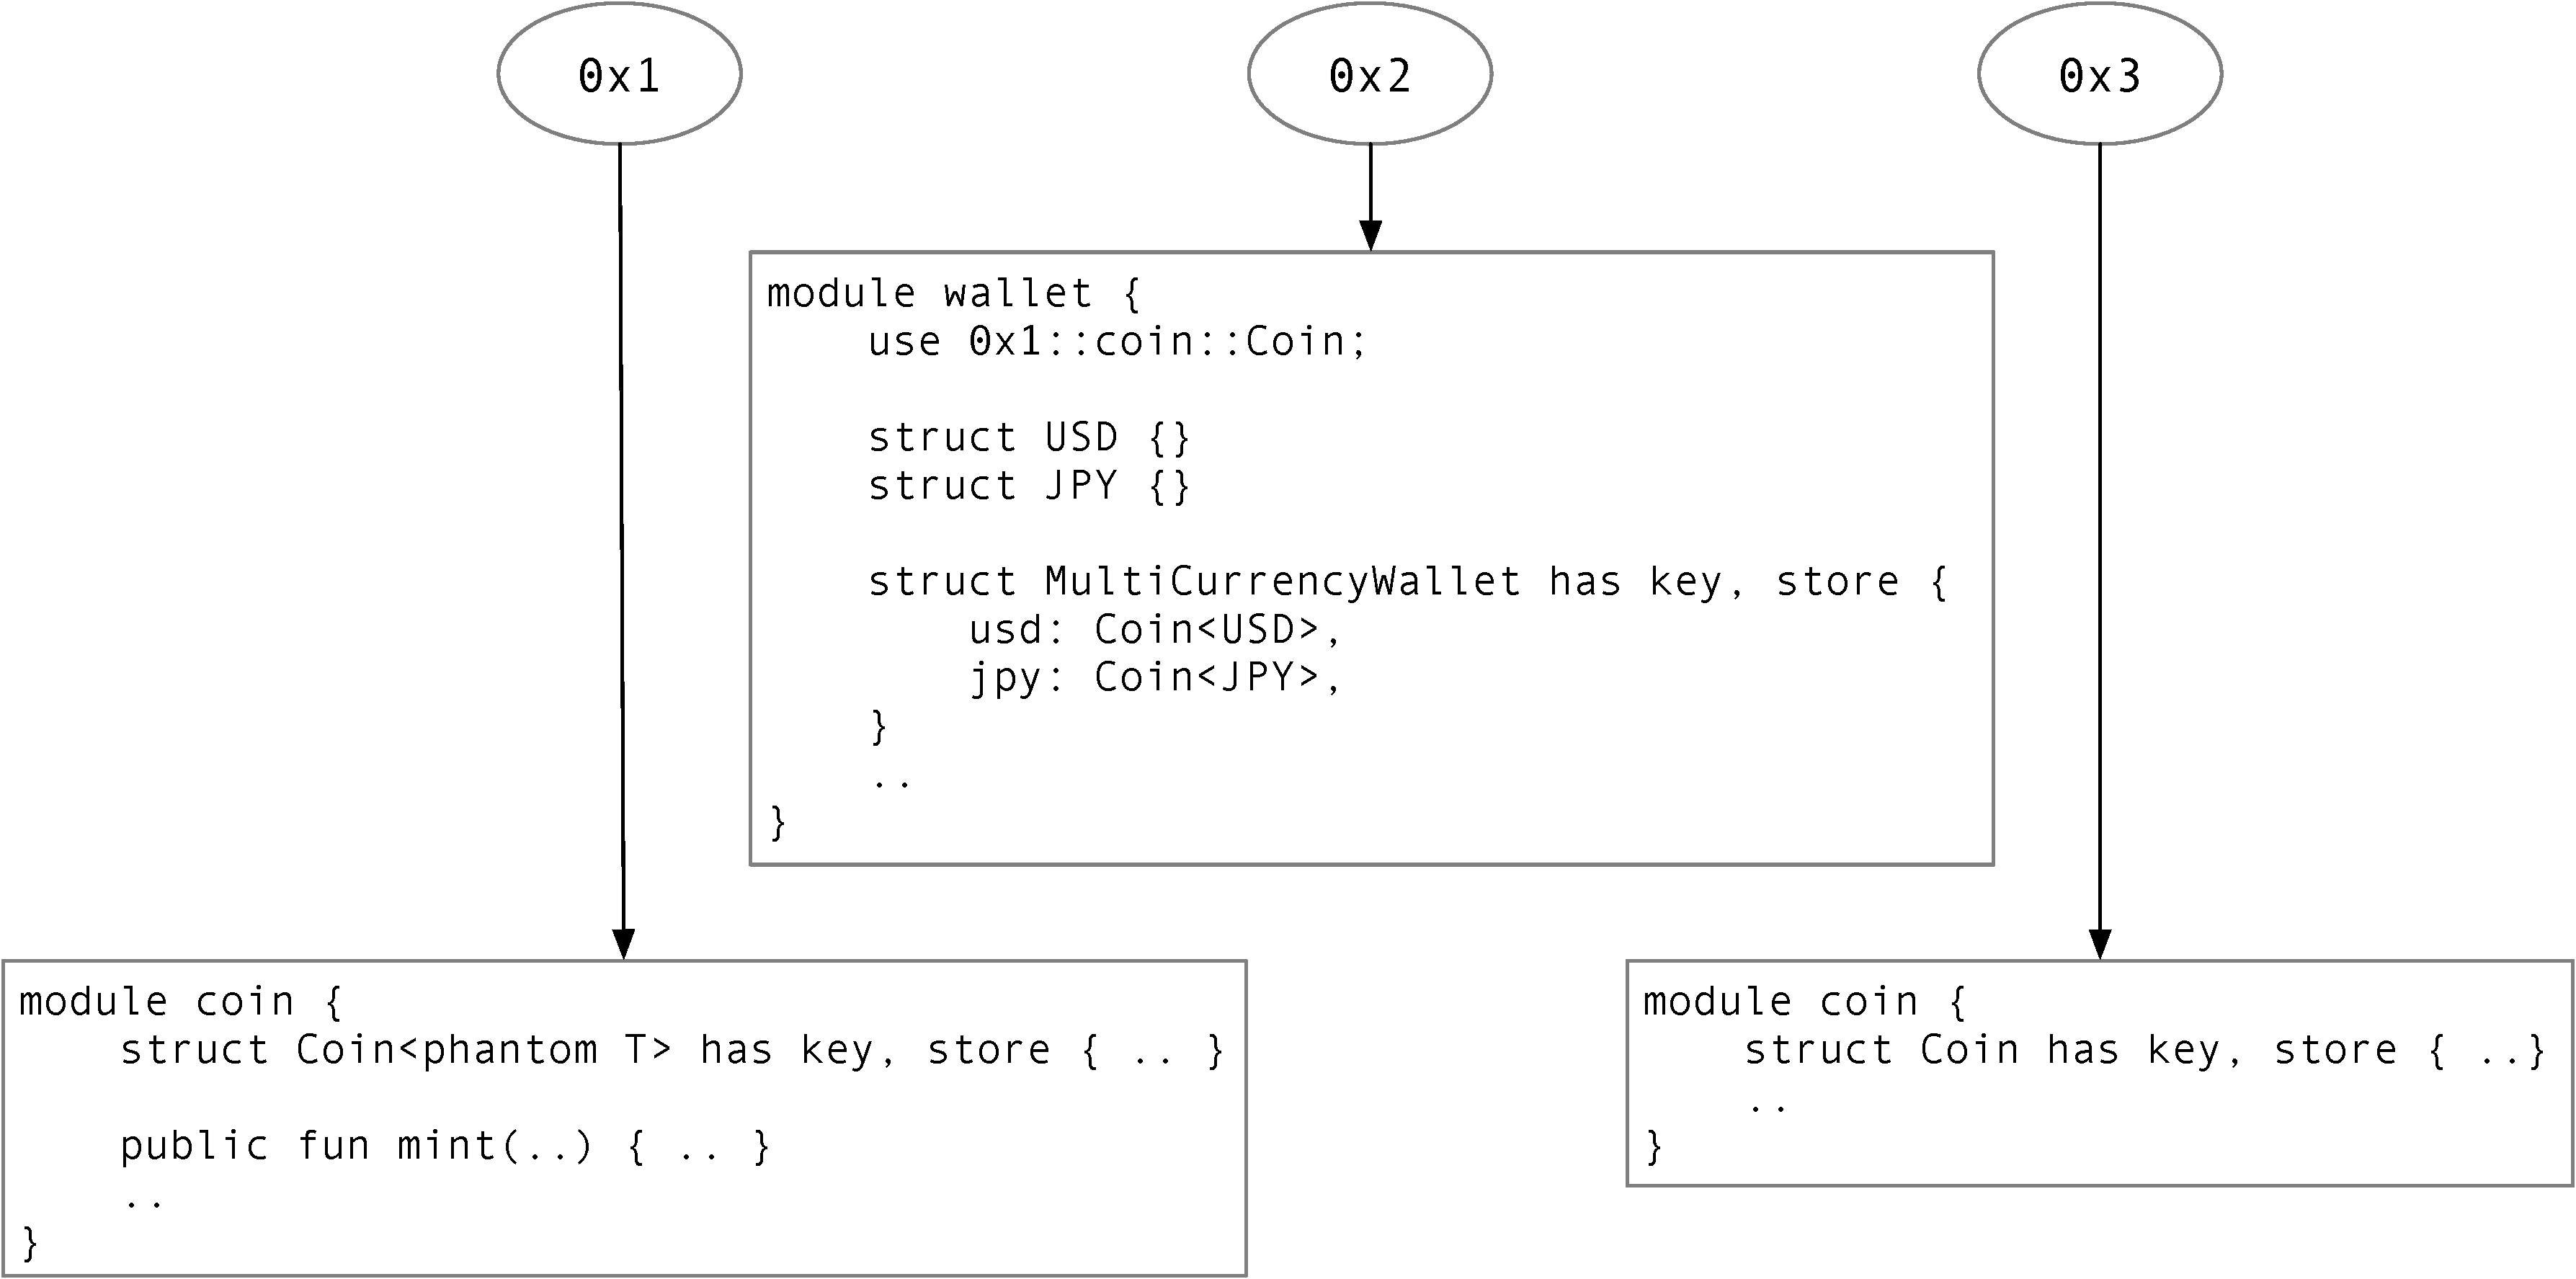
\includegraphics[width=0.85\textwidth]{move_1.pdf}
\caption{\label{fig:move_modules}オンチェーンMoveモジュールの例}
\end{figure}

\subsection{Moveモジュール}
\label{sec:move_modules}

Moveモジュールは、データ型(構造体)と手続きを宣言したMoveバイトコードを含みます。モジュールの識別は、モジュールが宣言されているアカウントのアドレスとモジュール名で行います。例えば、図\ref{fig:move_modules} の最初の通貨モジュールの識別子は \mintinline{rust}{0x1::coin} です。モジュールは、図\ref{fig:move_modules} のウォレットモジュールのように、他のオンチェーンモジュールに依存することができ、コードの再利用が可能になります。

つまり、各アカウントは最大で一つのモジュールを任意の名前で宣言することができます。例えば、図\ref{fig:move_modules}のアドレス0x1にあるアカウントは、\mintinline{rust}{coin}という名前の別のモジュールを宣言することができません。一方、アドレス  \mintinline{rust}{0x3} のアカウントは \mintinline{rust}{coin} という名前のモジュールを宣言することができ、このモジュールの識別子は \mintinline{rust}{0x3::coin} となります。\mintinline{rust}{0x1::coin::Coin} と  \mintinline{rust}{0x3::coin::Coin} は異なる型であり、互換性はなく、共通のモジュールコードを使用することもできないことに注意してください。一方、\mintinline{rust}{0x1::coin::Coin<0x2::wallet::USD>} と  \mintinline{rust}{0x1::coin::Coin<0x2::wallet::JPY>}  は同じ汎用型の異なるインスタンスで、互換性を持って使用することはできませんが、共通のモジュールコードを使用することはできます。

モジュールは、同じアドレスにあるパッケージにまとめられます。このアドレスの所有者は、バイトコードとパッケージのメタデータを含むパッケージを全体としてオンチェーンに公開します。パッケージのメタデータは、パッケージがアップグレード可能か、不変かを決定します。アップグレード可能なパッケージでは、アップグレードが許可される前に互換性チェックが行われます。既存のエントリポイント関数を変更してはならず、リソースをメモリに保存してはなりません。ただし、新しい関数やリソースを追加することは可能です。

Aptosブロックチェーンのコアライブラリと構成からなるAptosフレームワークは、モジュールの通常のアップグレード可能なパッケージとして定義されています(セクション \ref{subsec:network_governance}参照)。

\subsection{リソース} 
\label{subsec:resources}

モジュールと同様に、アカウントアドレスにもデータ値を関連付けることができます。各アカウントアドレス内では、値はそのタイプによってキーが付けられており、各タイプの最大1つの値がアカウントに属しています。図\ref{fig:move_data} はその例です。アドレス0x50には1つの値が格納され、\mintinline{rust}{0x3::coin::Coin} が完全修飾された値です。コインが完全修飾型です。 \mintinline{rust}{0x3} はコインモジュールが格納されているアドレス、 \mintinline{rust}{coin}はモジュール名、 \mintinline{rust}{Coin} はデータ型名です。汎用型の値も許容され、異なるインスタンス化されたものは異なる型として扱われます。これは拡張性のために不可欠であり、異なるインスタンスで同じ機能コードを共有することができます。

値の変更、削除、公開のルールは、データ型を定義するモジュールに記述されます。Moveの安全性と検証ルールにより、他のコードやエンティティが他のモジュールで定義されたデータ型のインスタンスを直接作成、変更、削除することを防ぐことができます。

\begin{figure}
\centering
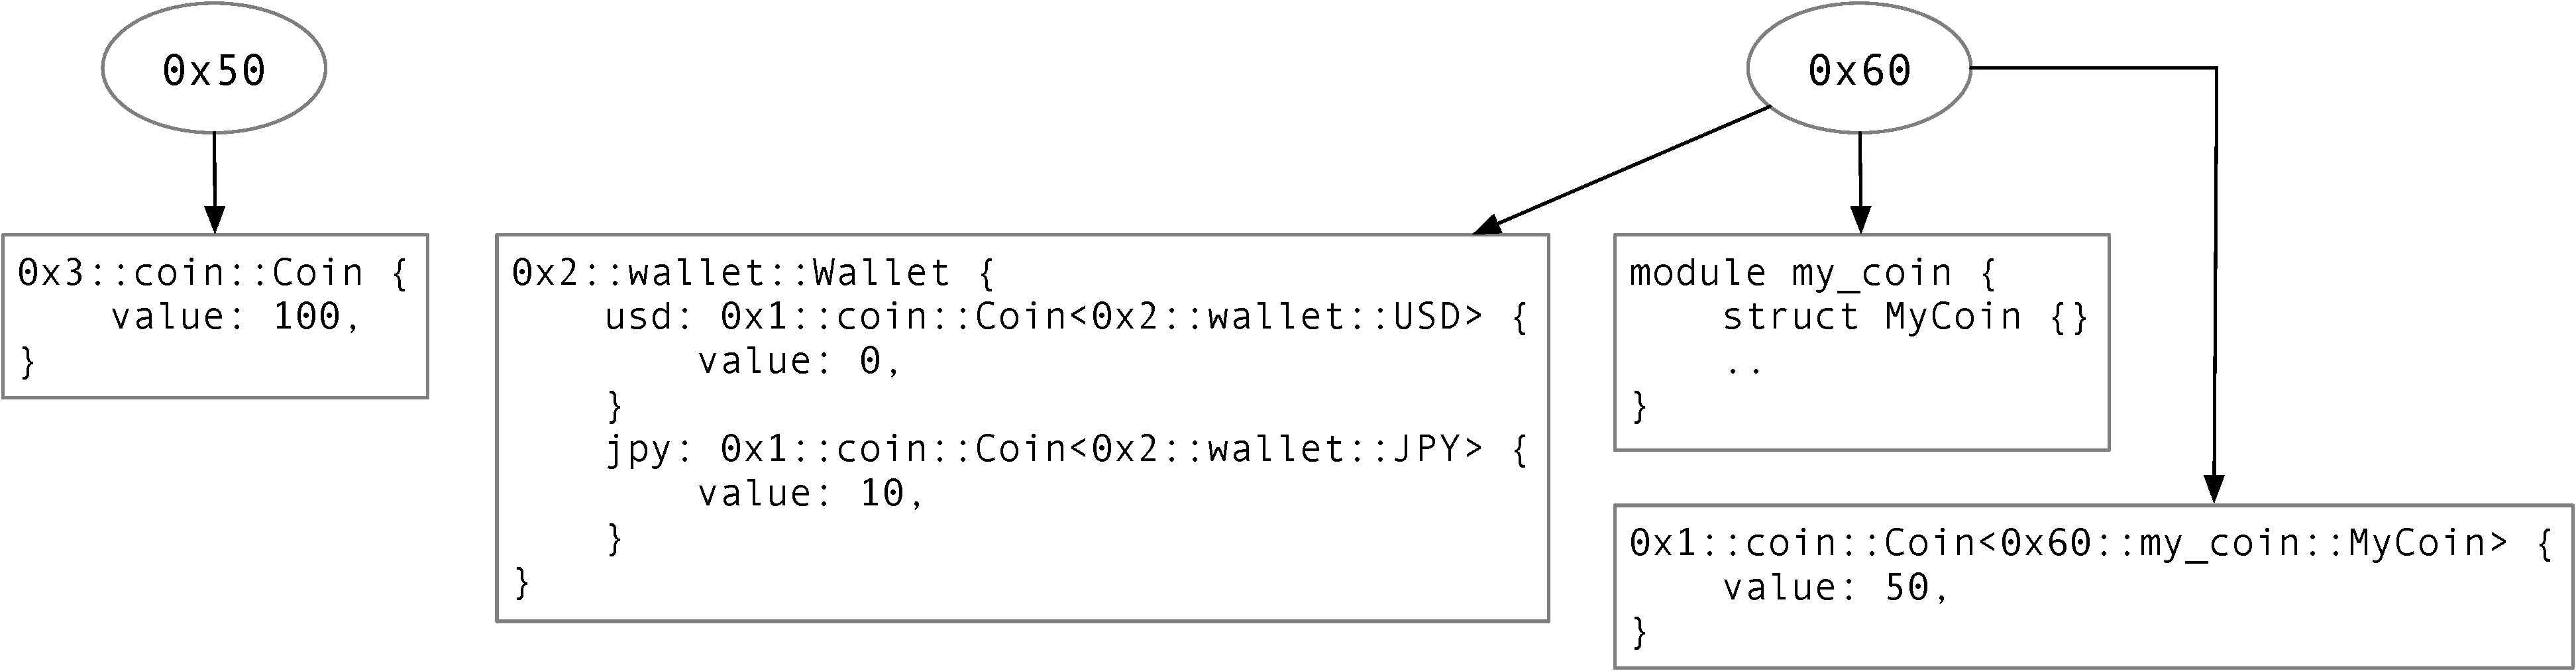
\includegraphics[width=1.0\textwidth]{move_2.pdf}
\caption{\label{fig:move_data}オンチェーンデータの例}
\end{figure}

アドレスの下に各タイプのトップレベルの値を1つだけ持つことは、一見制限的に聞こえるかもしれません。しかし、プログラマは他のデータを内部フィールドとするラッパータイプを定義することで、この制限を回避できるため、実際には問題にはなりません。図~\ref{fig:move_data}の\mintinline{rust}{Wallet} 構造体は、ラッパー型の使用方法の一例です。

また、すべてのデータ型がオンチェーンに格納できるわけではないことにも注意が必要です。データインスタンスをトップレベルの値として認定するには、そのデータ型に\mintinline{rust}{キー} 機能が必要です。同様に、ネストされた値にはストア能力が必要です。両方の能力を持つデータ型は、\emph{リソース}とも呼ばれます。

\subsection{元帳状態}
\label{sub:ledger_state}

Move仮想マシン(Move VM)の観点から、各勘定は値のセットとキー-値データ構造で構成されます。これらのデータ構造は\emph{テーブルエントリー}と呼ばれ、BCS(Binary Canonical Serialization)形式で保存されます。このデータレイアウトにより、開発者は、多数のアカウントに複製された少量のデータや、少数のアカウントに保存された大量のデータに対して効率的に動作するスマートコントラクトを記述することができます。Moveモジュールは、アカウントデータと同様に、独立した名前空間の下に格納されます。Genesis ledger stateは、ブロックチェーン初期化時のアカウントとその関連する状態の初期セットを定義します。

発売当初は、Aptosブロックチェーンは単一の台帳状態によって表されます。しかし、採用が進み技術が発展するにつれ、Aptosはシャードの数をスケールアップしてスループットを高め(つまり、複数の元帳状態を可能にし)、シャード間で資産を移動またはアクセスするトランザクションをサポートする予定です。各元帳の状態は、特定のシャードのすべてのオンチェーン資産を維持し、ストレージへのアクセスにほぼ固定費を提供する、きめの細かいキーバリューデータストアで同じアカウントモデルを提供します。

\section{安全なユーザーエクスペリエンス}
\label{sec:user}

何十億ものインターネットユーザーにアクセスするために、web3のユーザーエクスペリエンスは安全でアクセスしやすいものでなければなりません。以下のセクションでは、Aptosブロックチェーンが提供する、この目標に向けたいくつかの革新的な技術について説明します。

\subsection{取引の実行可能性保護}
\label{subsec:transaction_replay_protection}

取引に署名することは、署名者がその取引をブロックチェーンにコミットし実行することを承認することを意味します。時折、ユーザーは意図せず、または自分の取引が操作される可能性のあるすべての方法を十分に考慮せずに取引に署名することがあります。このリスクを減らすため、Aptosブロックチェーンはすべての取引の実行可能性を制約し、署名者を無制限の有効性から保護します。現在、Aptosブロックチェーンが提供する保護は、送信者のシーケンス番号、取引の有効期限、指定されたチェーン識別子の3種類です。
\begin{itemize}
 \item トランザクションのシーケンス番号は、各送信者のアカウントに対して正確に1度だけコミットすることができます。その結果、送信者は、現在のアカウントのシーケンス番号$\geq$取引 $t$ のシーケンス番号の場合、 $t$ はすでにコミットされているか、 $t$ がコミットされることはない(  $t$ が使用するシーケンス番号はすでに他の取引によって消費されているため)ことを観察することができます。

 \item ブロックチェーンの時間は、セクション\ref{subsubsec:blockchain_time}で説明したように、高い精度と周波数(通常はサブ秒)で進みます。 ブロックチェーン時間が取引 $t$ の有効期限を超えた場合、同様にtは既にコミットされているか、あるいは$t$ がコミットされることはありません。

 \item すべての取引は、悪意のあるエンティティが異なるブロックチェーン環境間(例えば、テストネットとメインネット間)で取引を再生することを防ぐために、指定されたチェーン識別子を持ちます。

\end{itemize}

\subsection{Moveベースのキー管理}
\label{sub:move_based_key_management}

セクション\ref{sec:accounts}で説明したように、Aptosアカウントはキーローテーションをサポートしており、秘密鍵の侵害、長距離攻撃、および既存の暗号アルゴリズムを破る可能性がある、将来の進歩に関連するリスクを減らすのに役立つ重要な機能となっています。さらに、Aptosアカウントは、新しいハイブリッドカストディモデルを可能にするのに十分な柔軟性を持っています。そのようなモデルでは、ユーザーはアカウントの秘密鍵を回転させる能力を、1人以上のカストディアンや他の信頼できるエンティティに委譲することができます。Moveモジュールは、これらの信頼できるエンティティに、特定の状況下で鍵を回転させる権限を与えるポリシーを定義することができます。例えば、エンティティは多くの信頼できる当事者によって保持される$k$-out-of-$n$ multi-sigキーによって表され、ユーザーの鍵紛失を防ぐために鍵回復サービスを提供するかもしれません(例えば、現在ビットコインの20\%が回復不能なアカウントにロックアップされています \cite{lost_passwords})。

さらに、多くのウォレットは、クラウドインフラへの秘密鍵のバックアップ、マルチパーティ計算、ソーシャルリカバリーなど、様々な鍵回復スキームをサポートしていますが、それらは通常、ブロックチェーンをサポートせずに(すなわちオフチェーンで)実装されています。その結果、各ウォレットは独自の鍵管理インフラを実装する必要があり、関連する操作はユーザーにとって不透明なものとなっています。対照的に、Aptosブロックチェーン層で鍵管理機能をサポートすると、すべての鍵関連操作の完全な透明性が得られ、豊富な鍵管理機能を持つウォレットの実装がより簡単になります。

\subsection{事前署名のトランザクションの透明性}
\label{sub:pre-signing_transaction_transparency}

今日、ウォレットは署名するトランザクションについてほとんど透明性を提供していません。その結果、ユーザーはしばしば簡単に騙されて、資金を盗み、壊滅的な結果をもたらすかもしれない悪意のある取引に署名してしまいます。これは、各取引によってアクセスされる、すべてのオンチェーンデータを列挙する必要があるブロックチェーンにも当てはまります。そのため、現在、ユーザーのセーフガードはほとんどなく、ユーザーはさまざまな攻撃にさらされやすくなっています。

これに対処するため、Aptosエコシステムは、\emph{トランザクションの事前実行}のためのサービスを提供します:これは、署名の\emph{前}にトランザクションの結果を(人間が読める形で)ユーザーに説明する予防措置です。これと、過去の攻撃や悪意のあるスマートコントラクトの既知の履歴を組み合わせることで、不正を減らすことができます。さらに、Aptosでは、ウォレットが実行中の取引に制約を指示することも可能です。これらの制約に違反すると、悪意のあるアプリケーションやソーシャルエンジニアリング攻撃からユーザーをさらに保護するために、トランザクションが中止されることになります。

\subsection{実用的なライトクライアントプロトコル}
\label{practical_light_client_protocols}

ブロックチェーンクライアントとサーバー間の信頼を確立するためにAPIプロバイダーのTLS/SSL証明書のみに依存することは、クライアントを十分に保護することができません。有効な証明書がある場合でも、ウォレットとクライアントは提示されるデータの真正性と完全性に関して何の保証もありません。その結果、APIプロバイダーは不正確な、または悪意のあるブロックチェーンデータを返し、第三者を欺き、二重支出攻撃を行う可能性があります。

これを防ぐため、Aptosは状態証明とライトクライアント検証プロトコルを提供し、ウォレットとクライアントが信頼できない第三者サーバーから提示されるデータの妥当性を検証するために使用できます。さらに、セクション\ref{subsubsec:period_state_certification}のタイムスタンプベースの状態証明を活用することで、ライトクライアントは常にアカウント状態の鮮度(例えば、数秒以内)の厳しい境界を保証することができ、ネットワーク構成の変更(\emph{エポック変化})を追跡するか、現在の信頼できるチェックポイント(\emph{ウェイポイント})を使用して最新状態に保つだけでよいのです\cite{waypoints}。高頻度のタイムスタンプと安価な状態証明を組み合わせることで、Aptosブロックチェーンはクライアントにセキュリティ保証の向上を提供します。

さらにAptosノードは、チェーン上の特定のデータやアカウントを対象とした証明へのサブスクリプションを可能にするために、さらに細かく調整できるリッチで高性能なストレージインターフェースも公開します。これは、フルノードの実行や相当数のトランザクションを処理する必要なく、最小限の検証可能なデータを保持するためにライトクライアントによって活用されることができます。

\section{パイプライン化、バッチ処理、並列トランザクション処理}
\label{sec:pipelining_batching}

スループットを最大化し、並行性を高め、エンジニアリングの複雑さを軽減するために、Aptosブロックチェーン上のトランザクション処理は、個別のステージに分割されています。各ステージは完全に独立しており、個別に並列化可能で、現代のスーパースカラー・プロセッサー・アーキテクチャに似ています。これは性能面で大きな利点をもたらすだけでなく、Aptosブロックチェーンがバリデータとクライアントの新しい相互作用のモードを提供することを可能にします。例えば、以下のようなものです。
\begin{itemize}
 \item 特定のトランザクションが永続化されたトランザクションのバッチに含まれる場合、クライアントに通知することができます。永続化された有効なトランザクションは、間もなくコミットされる可能性が高いです。

 \item 永続化されたトランザクションのバッチが注文されたときに、クライアントに通知することができます。したがって、実行されたトランザクション出力を決定する待ち時間を短縮するために、クライアントは、バリデータがリモートで実行を完了するのを待つのではなく、ローカルでトランザクションを実行するように選択することができます。

 \item クライアントは、バリデータによる認証済みトランザクションの実行を待ち、 認証済み結果に対して状態同期を実行することを選択できます(たとえばセクション \ref{sub:state_sync}を参照)。

\end{itemize}

Aptosのモジュール設計は、単一のモノリシックなアーキテクチャではなく、個々のモジュールに変更を加えることができるため、開発速度を助け、より速いリリースサイクルをサポートします。同様に、モジュール設計は、バリデータを単一マシンから拡張するための構造化されたパスを提供し、追加の計算、ネットワーク、およびストレージリソースへのアクセスを提供します。図 \ref{fig:pipeline}は、さまざまな処理段階におけるトランザクションのライフサイクルを示しています。

\begin{figure}
\centering
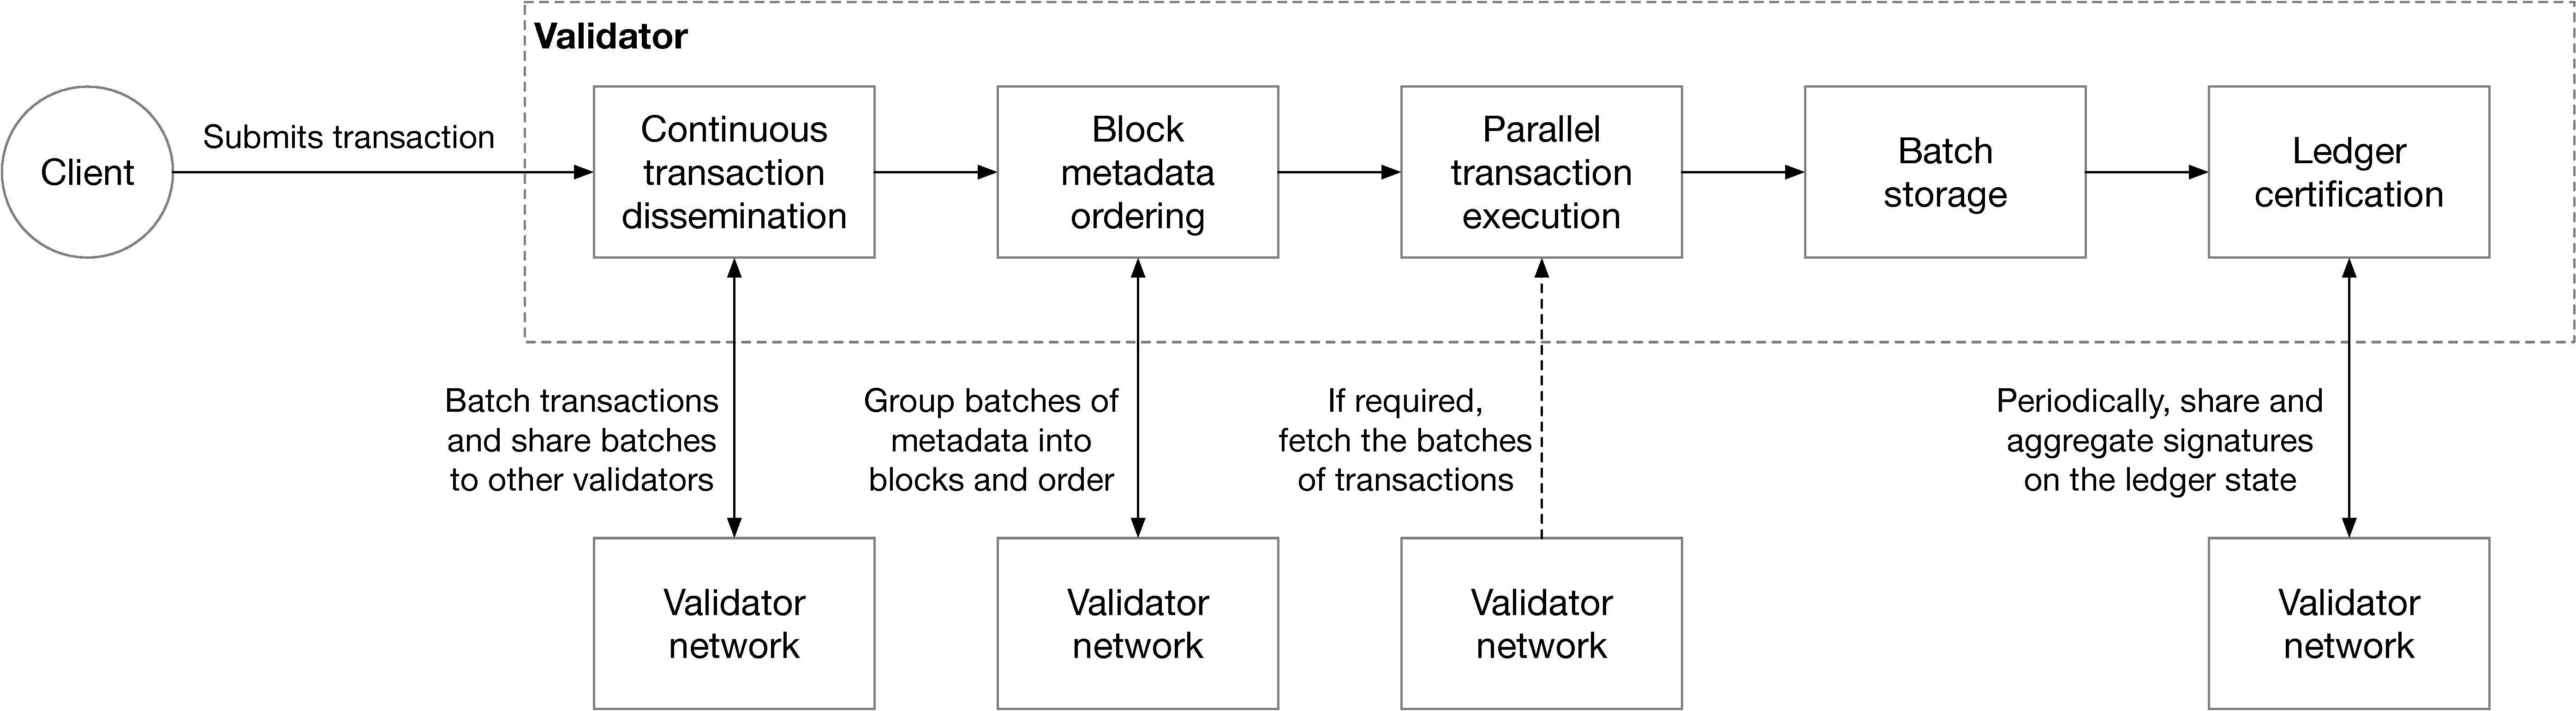
\includegraphics[width=1.0\textwidth]{pipeline.pdf}
\caption{\label{fig:pipeline}トランザクション処理のライフサイクル。すべてのステージは完全に独立しており、個々に並列化可能である。}
\end{figure}

\subsection{バッチ処理}
\label{sub:batch_processing}

バッチ処理は、Aptosブロックチェーンにおける操作のあらゆる段階の一部である重要な効率最適化です。取引は、取引の普及中に各バリデータによってバッチにグループ化され、バッチはコンセンサス中にブロックに結合されます。また、実行、保存、台帳認証の各フェーズでは、バッチ処理により、順序の入れ替え、演算の削減(重複計算や署名検証など)、並列実行の機会が提供されます。

トランザクションをバッチにまとめると、例えば、配信を実行する前にトランザクションのバッチを蓄積するために200ミリ秒待つなど、わずかな遅延が発生する可能性があります。しかし、バッチングは最大待ち時間や最大バッチサイズに関して簡単に設定できるため、分散型ネットワークは待ち時間と効率性を自動的に最適化することができます。バッチングはまた、トランザクションに優先順位をつけ、熱狂的なクライアントからの意図しないサービス拒否(DoS)攻撃を避けるための効率的な手数料市場も可能にします。

\subsection{継続的な取引の普及}
\label{continuous_txn_dissemination}

Narwhal \& Tusk \cite{narwhal_tusk}の主要な洞察に従い、Aptosブロックチェーンにおける取引の普及はコンセンサスから切り離されています。バリデータはトランザクションのバッチを継続的に互いに配信し、利用可能なネットワーク資源をすべて同時に利用します。バリデータ $v$ によって配信された各バッチは永続化され、バッチダイジェストへの署名が $v$ に送り返されます。セクション \ref{subsec:block_metadata_ordering}で定義された合意要件に従い、バッチダイジェストへの任意の $2f+1$ ステーク加重署名は、可用性の証明(PoAv)を形成しています。この証明は、少なくとも $f+1$ のステークに応じた誠実なバリデータが バッチを保存していることを保証するものであり、したがって、すべての誠実なバリデータが実行前にそれを取得することができるようになります。

トランザクションのバッチを無限に持続させると、バリデータが記憶装置を使い果たしてクラッシュすることで、DoS攻撃ベクトルを開くことができます。これを防ぐため、トランザクションの各バッチには関連するタイムスタンプを設定します。バッチのタイムスタンプは、各バリデータでの効率的なガベージコレクションを可能にします。さらに、バリデータごとのクォータメカニズムは、潜在的なビザンチン攻撃のような極端な状況においても、バリデータの容量不足を防ぐように設計されています。バッチはまた、安定したストレージへの永続化に合意する前に検証されるサイズ制約を持ちます。最後に、トランザクションの重複を排除しキャッシュするためのいくつかの最適化により、ストレージコストを削減し、並列実行エンジンとの性能の良い統合を保証します。

\begin{figure}
\centering
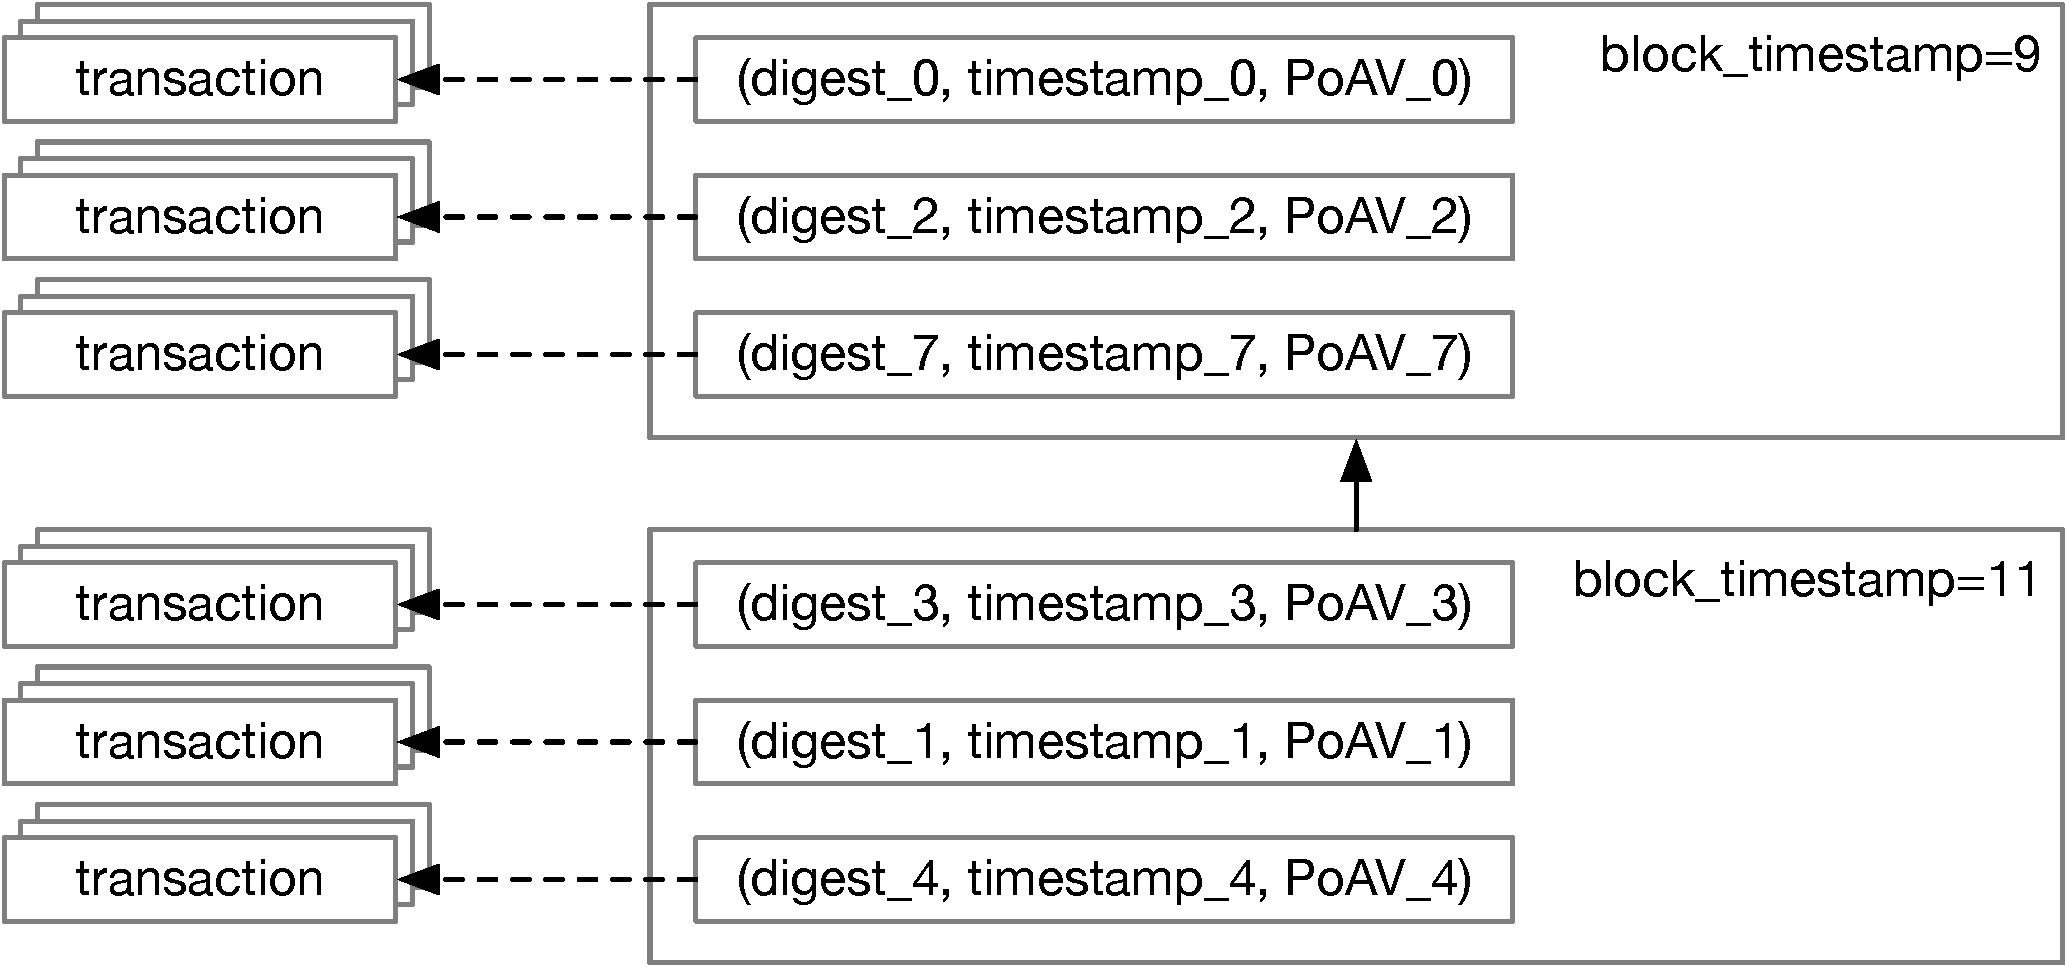
\includegraphics[width=0.8\textwidth]{ordering.pdf}
\caption{\label{fig:block}ブロックメタデータの順序付けは、トランザクションの配信とは独立して行われる。}
\end{figure}

\subsection{ブロックメタデータの順序付け}
\label{subsec:block_metadata_ordering}

一般的な誤解の一つは、コンセンサスが遅いため、ブロックチェーンのスループットとレイテンシー(遅延時間)の主要なボトルネックになっているというものです。Aptosブロックチェーンの重要な革新的技術の一つは、取引の普及、取引の実行/保存、元帳の証明など、合意に関連しない作業を合意段階から切り離すことです。取引の普及を合意段階から切り離すことで、非常に低い帯域幅(ブロックメタデータと証明のみ)で注文を行うことができ、高い取引スループットと最小限のレイテンシーを実現しています。

今日、Aptosブロックチェーンは、楽観的に反応するBFTコンセンサスプロトコルであるDiemBFTv4 \cite{diembft_v4}の最新版を活用しています。一般的なケースでのコンセンサスは、2回のネットワーク往復で済み(往復時間は世界中で通常300ミリ秒未満)、リーダーの評価メカニズム \cite{be_aware}を通じて欠陥のあるバリデータに動的に調整されます。オンチェーンリーダーレピュテーションメカニズムは、ウィンドウ内でブロックのコミットに成功したバリデータを昇格させ、参加していないバリデータを降格させます。この新しいメカニズムは、分散環境における性能を大幅に向上させ、それに応じて適切なインセンティブのためのインフラを提供し、失敗したバリデータがスループットとレイテンシーに与える影響を迅速に最小化します。

DiemBFTv4は部分的な同期のもとで有効性を保証し、非同期のもとで安全性を保証します。このときバリデータの総ステークが $\geq 3f+1$ であり、ステークに応じた最大 $f$ の欠陥バリデータが存在します。DiemBFT04は、2019年以降、数十のノードオペレータとマルチウォレットエコシステムを使用して、いくつかのイテレーションで広範囲にテストされています。また、私たちの最近の研究(例えば、Bullshark \cite{bullshark})や、ブロックメタデータの順序と最終性を決定するためにブロック履歴と関連する通信に依存する他のプロトコルの実験も行っています。

図\ref{fig:block}に示すように、コンセンサスブロックと提案タイムスタンプはリーダーが提案し、他のバリデータによって合意されます。各コンセンサスブロックには、バッチメタデータとプルーフのみが含まれることに注意してください。実際のトランザクションはブロック内に必要ありません。PoAVはトランザクションのバッチが注文後の実行フェーズで利用可能になることを保証しているからです(セクション~\ref{continuous_txn_dissemination}参照)。バリデーターは、証明とブロックメタデータの基準を満たした後、リーダーの提案に投票できます(例: 提案タイムスタンプ $\le$ ブロック有効期限)。

\subsubsection{ブロックチェーンの時間}
\label{subsubsec:blockchain_time}

Aptosブロックチェーンは、提案されたすべてのブロックと、それに対応するそのブロック内のすべての取引について、おおよその、合意された、物理的なタイムスタンプを採用します。このタイムスタンプは、多くの重要なユースケースを可能にします。例えば、以下のようなものです:

\begin{itemize}
 \item スマートコントラクトにおける時間依存のロジックです。例えば、あるオークションの入札はすべて木曜日の正午までに受けなければならない、というエンコードを開発者が希望しているとします。

 \item オラクルはオンチェーンデータを公開するため、イベントの関連付けや実世界のデータからの遅延を処理するために、正確で信頼できるオンチェーンタイムスタンプが必要とされます。

 \item クライアントは、ブロックチェーンに対して自分がどれだけ最新であるかを見分けることができます。セキュリティ上の理由から、古いデータや長距離攻撃を避けるために、クライアントはアカウントの状態が更新されたときの高精度のタイムスタンプにアクセスできる必要があります。

 \item 信頼性の高いタイムスタンプでブロックチェーンを監査することで、法的に強制される支払いが期待される要件を満たすことを保証するなど、オフチェーンイベントとの強い相関性を実現します。

 \item トランザクションの有効期限は、直近のコミットされたタイムスタンプに基づきます。クライアントのトランザクションに対する追加の保護として、クライアントはトランザクションの有効期限を選択することができます。セクション \ref{subsec:transaction_replay_protection}で説明されています。

\end{itemize}

Aptosブロックチェーンは、ブロック内の全取引のタイムスタンプに関して、以下の保証を提供します。

\begin{itemize}
 \item ブロックチェーンでは、時間は単調に増加します。つまり、$B1 < $ block $B2$ であれば $B1.Time < B2.Time$ となります。

 \item ある取引ブロックがタイムスタンプ $T$で合意された場合、少なくとも $f+1$ 人の誠実なバリデータはTが過去であると判断しています。正直なバリデータは、自身のクロック $\ge$ タイムスタンプ $T$のときのみ投票します。 \ref{continuous_txn_dissemination}を参照。

 \item ある取引ブロックがタイムスタンプ $T$で署名のクォーラムを満たす場合、正直なバリデ ータはそのようなブロックを提供しません。 バリデータは、自身のクロック $\ge$ タイムスタンプ $T$ になるまで、 そのようなブロックを他のバリデータに提供しません。
 
 \end{itemize}

最新のタイムスタンプはコミットされたブロックごとに更新され、そのブロック内のすべてのトランザクションのタイムスタンプとして使用されます。ネットワークが同期の場合、トランザクションのブロックはネットワークの1往復ごとにコミットされ、高速更新と高い信頼性を持つクロックを提供します。 トランザクションのブロック内の順序は、必要に応じてより細かい粒度を決定することができます。

\subsection{トランザクションの並列実行}
\label{subsec:parallel_transaction_execution}

コンセンサスブロックメタデータが発注されると、どのバリデータ、フルノード、 クライアントでもトランザクションを実行することができます。少なくとも $2f+1$ stakeの重み付けをしたバリデータが、提案されたバッチのトランザクションを検証可能な状態で持続しています。トランザクションの配布は継続的に行われるため、時間の経過とともに、誠実なバリデ ータはトランザクションバッチをさらに受信することになります。もしある誠実な検証者が、実行段階に達するまでに注文したバッチの取引を受け取っていない場合、少なくとも $f+1$ 人のステークウェイト付きバリデータ( $\ge$ ステークウェイト付き PoAV署名者)が誠実であることを知っているので、 $2f+1$ 人のステークウェイト付きバリデータから取引をダウンロードすることが可能です。

ブロックチェーンの重要な目標は、可能な限り並列実行を可能にすることです。Aptosブロックチェーンは、データモデルと実行エンジンの両方からこの方向性を前進させます。

\subsubsection{並列データモデル}

Moveデータモデルは、データとモジュールのグローバルアドレッシングをネイティブにサポートします。データやアカウントに重複する競合がないトランザクションは、並行して実行することができます。Aptosブロックチェーンで使用されるパイプライン設計を考えると、トランザクションのグループを並べ替えることで競合の数を減らし、それによって並行性を向上させることができます。

トランザクションが同じオンチェーン値のセットを変更する場合でも、トランザクション実行プロセスの多くを並列化することが可能です。Aptosブロックチェーンは、変更されたアカウント状態ではなく、アカウント状態への変更を記述する新しい概念、\emph{デルタライト}を導入しています(例えば、最終値を単純に決定するのではなく、整数をインクリメントします)。すべてのトランザクション処理を並行して完了し、その後、デルタライトを競合する値に対して正しい順序で適用することで、決定論的な結果を確保することが可能です。

Aptosブロックチェーンは、時間をかけて、並行性を向上させる方法(例えば、読み取り/書き込みヒントを活用する)でデータモデルを強化し、また人間工学を改善し、開発者がオンチェーン値を作成、変更、構成することをより自然にすることを継続します。Moveは、言語レベルだけでなく、プラットフォーム固有の機能によって、このような改善を柔軟に行うことができます。

\begin{figure}
\centering
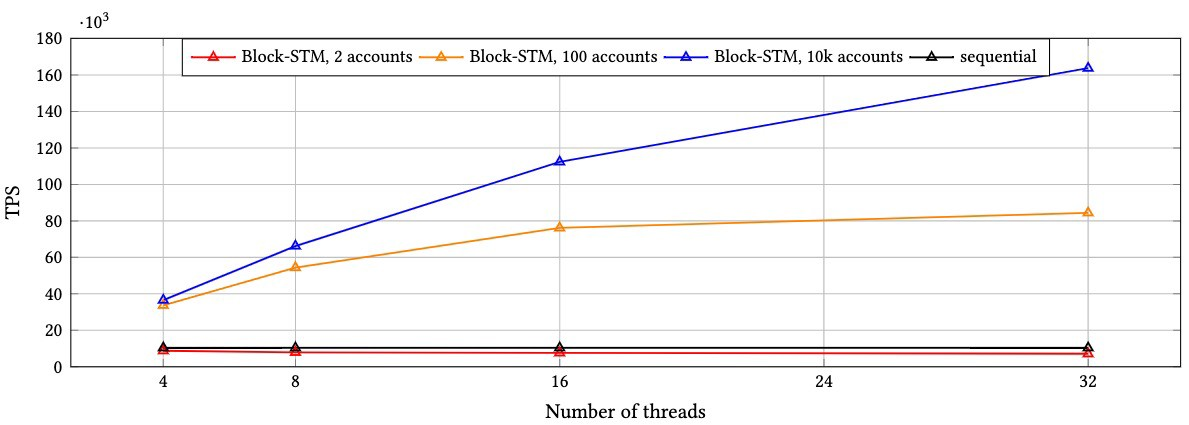
\includegraphics[width=0.95\textwidth]{perf.jpg}
\caption{\label{fig:perf}Block-STM(コンポーネントのみ)ベンチマークで、競合の度合いを変えて物理コア数を比較。}
\end{figure}

\subsubsection{並列実行エンジン}

Block-STMの並列実行エンジンは、特定の順序が与えられた場合に最大の並列性を可能にする楽観的同時実行制御とともに、順序付けられた一連のトランザクションの競合を検出して管理します \cite{block_stm}。

トランザクションのバッチは楽観的に並列実行され、実行後に検証されます。検証に失敗すると、再実行されます。Block-STMは書き込みと書き込みの競合を避けるため、複数バージョンのデータ構造を使用します。同じ場所へのすべての書き込みは、そのトランザクションIDと書き込みトランザクションが最適に再実行された回数を含むバージョンと一緒に保存されます。トランザクション $tx$ がメモリロケーションを読み取るとき、あらかじめ設定された順序で $tx$ の前に現れる最も高いトランザクションによってこのロケーションに書き込まれた値を、関連するバージョンとともにマルチバージョンデータ構造から取得します。

Block-STMは、すでにAptosブロックチェーンに統合されています。Block-STMの性能の可能性を完全に理解するために、インメモリデータベースを用いた実行のみの(エンドツーエンドではない)独立したベンチマークとして、非自明なピアツーピアMoveトランザクション(すなわち、トランザクションごとに8回の読み取りと5回の書き込み)の実験を実行しました。図 \ref{fig:perf}では、Block-STMの実行結果を示しています。各ブロックは10kトランザクションを含み、アカウント数によってコンフリクトとコンテンションのレベルが決定されます。

Block-STMは、低競争下では32スレッドの逐次実行に比べて16倍のスピードアップを達成し、高競争下では8倍以上のスピードアップを達成しています。Block-STMは、ブロックチェーン分野の他の並列実行エンジンとは異なり、あらゆるワークロードから固有の並列性を動的かつ透過的に(ユーザーからのヒントなしに)抽出することができます。読み書きの対象となるデータ位置を前もって知っておく必要がある並列実行環境と比較して、Block-STMはより複雑なトランザクションを同時にサポートすることができます。この特性により、トランザクションの数が少なくても効率的で、コストを削減し、ユーザーに低遅延を提供することができます。おそらく最も重要なことは、アトミックトランザクションを複数の小さなトランザクションに分割することで、複雑な状態の結果を伴う単一トランザクションのall-or-nothingセマンティクスを壊すことです。Block-STMで表現力豊かなトランザクションセマンティクスと並列実行を組み合わせることで、開発者は両者の長所を享受することができます。

ブロックメタデータの順序付けステップは、並列実行フェーズでのトランザクションの再順序付けを妨げないことに注意してください。トランザクションは、並列実行の同時実行性を最適化するために、1つまたは複数のブロックにわたって並べ替えが可能です。唯一の要件は、並べ替えはすべての誠実なバリデータに対して決定論的でなければならないことです。並列実行を最適化すると同時に、並べ替えにランダム性を持たせることで、性能を向上させることができ、また最大抽出値 (MEV) 技術による有益なバリデータの並べ替えを阻止できる可能性があります。このパイプライン化された設計には、「Order-then-reveal」MEV耐性戦略も組み込むことができます。

ブロックSTMとトランザクションの並べ替えは、実行の並列性を高めるための補完的な技術です。これらは、トランザクションの読み取り/書き込みアクセスヒントと組み合わせて、さらに並行性を高めることができます。

\subsection{バッチストレージ}

並列実行フェーズでは、グループ内の全トランザクションの書き込みセットが生成されます。これらの書き込みセットは、実行速度を最大化するためにメモリに保存され、次に実行されるブロックまたはブロックのセットのためのキャッシュとして使用されることができます。重複する書き込みは、安定したストレージに一度だけ書き込まれれば大丈夫です。バリデータがメモリ内の書き込みセットを保存する前に失敗した場合、ブロックメタデータの順序付け段階から並列実行を再開するだけで大丈夫です。書き込みセットのバッチ保存を並列実行のステップから切り離すことで、並列実行を効率的に行えるようになります。要約すると、書き込みセットをバッチ処理することで、ストレージ操作の回数を減らし、より効率的で大規模なI/O操作を利用することができます。

ライトセットキャッシングのために確保されるメモリ量は、マシンごとに手動で設定でき、自然なバックプレッシャーメカニズムを提供します。特定の I/O およびメモリ環境に合わせてチューニングするために、必要に応じてバッチの粒度を並列実行ブロックの粒度と異ならせることができます。

\subsection{台帳認証}

パイプラインのこの時点で、個々の検証者はコミットされたトランザクションのブロックに ついて新しい状態を計算しました。しかし、検証済みライトクライアントと状態の同期を効率的にサポートするために、Aptosブロックチェーンは、元帳の状態と同様に元帳の履歴のための元帳認証を実装しています。Aptosブロックチェーンの1つの重要な違いは、元帳認証がトランザクション処理のクリティカルパス上になく、必要であれば完全にアウトオブバンドで実行することも可能であるということです。

\subsubsection{台帳の履歴認証}
\label{subsubsec:ledger_history_certification}

バリデータは、トランザクションをその実行結果と共に、グローバルな認証済み台帳データ構造に追加します。トランザクション出力の一部は、Moveによってアクセス可能なグローバルな状態に対して行われた変更からなる状態書き込みセットです。このデータ構造の短い認証子は、新たに実行されたトランザクションのバッチを含む元帳履歴へのバインディングコミットメントです。トランザクションの実行と同様に、このデータ構造の生成は決定論的です。

各バリデータは、生成されたデータベースの新バージョンに対して、短い認証子に署名します。バリデータは最近の署名済み短認証子のセットを互いに共有し、クォーラム署名済み短認証子を一括して集約し、さらに最近のクォーラム署名済み短認証子を互いに共有します。

この集合署名を使用することで、クライアントはプロトコルのBFT特性に従って、データベースのバージョンが、完全で有効かつ不可逆な元帳の履歴を表していると信頼することができます。クライアントは、任意のバリデータ(またはフルノードなどのサードパーティのデータベース複製)に問い合わせてデータベースの値を読み取り、その結果を認証子と目的のデータの証明書を使用して検証することができます。

\subsubsection{定期的な状態の認証}
\label{subsubsec:period_state_certification}

Moveからアクセス可能なグローバルステートの全体は、台帳の履歴の要約と同様に、歴史のどの時点でも短い認証子に要約することが可能です。グローバル状態はランダムアクセスのため(追記のみの台帳履歴と異なり)、この認証の維持には大きなコストがかかります。とはいえ、データ構造を大量に一括して更新する場合、更新を並列に計算し、さらに個々の状態の値が変化したときに更新しなければならない部分の重複を利用することができます。Aptosブロックチェーンは、共有更新の重複を減らすために、意図的にグローバル状態を定期的に認証するだけです。

決定論的かつ設定された間隔の間、ネットワークは、その出力の一部としてグローバル状態の認証子を含む状態チェックポイントトランザクションを発行します。このようなバージョンは\emph{ステートチェックポイント}と呼ばれます。2つのチェックポイント間のギャップが大きいほど、トランザクションごとに状態認証データ構造を更新するための償却コストは低くなります。

状態チェックポイントを用いると、グローバルな状態をすべて保存することなく、チェックポイントから任意の状態値を信頼できる方法で読み出すことができます。この機能は、状態のインクリメンタルな同期、バリデータ間のシャード化されたストレージ、 ステートレスバリデータノード、ストレージに制約のあるライトクライアントなどの用途に有用です。

しかし、ステートチェックポイントは定期的に行われるため、元帳の状態の特定のバージョンに対する証明を得るには、欠落した状態の代替のための追加のトランザクションを実行するか、認証された元帳の履歴からそれらを含める証明を行う必要があります。

ステートチェックポイントは、元帳履歴の特定の取引バージョンに関連付けられ、それゆえ、セクション\ref{sec:pipelining_batching}で述べた取引バッチに関連付けられたタイムスタンプに束縛されます。タイムスタンプがあれば、ライトクライアントは証明されたステート値の最新性を理解することができます。タイムスタンプがなければ、ライトクライアントの証明は、はるか過去の状態の有効性しか保証できず、関連性の保証はほとんどありません。また、ステート証明のタイムスタンプは、過去のアクセスの追跡や監査目的(トークン備蓄の時間ごとの平均残高の計算など)に必要です。

ステートチェックポイントは、以前のステートチェックポイントと、それ以降のトランザクション出力における状態交替に基づいて導き出すことができます。したがって、ステートチェックポイントを安定したストレージに保存することは、トランザクション処理のクリティカルパスである必要はありません。また、ステートチェックポイントを永続化する際にも、有益なバッチング効果が存在します。最近のステートチェックポイント(というよりその間の差分)をメモリにキャッシュし、定期的なステートチェックポイントのみを安定したストレージにダンプすれば、ストレージ帯域の消費を大幅に抑えることができます。チェックポイントを永続化するために選択する方法は、認証済みデータ構造の計算には影響しません。したがって、これはノードごとの選択となります。ノードオペレータは、メモリ容量とストレージ帯域幅の適切なトレードオフを設定することができます。

\section{状態の同期化}
\label{sub:state_sync}

Aptosブロックチェーンは、エコシステムのすべての参加者に高スループット、低レイテンシーシステムを提供することを目的としています。その結果、ブロックチェーンは、ライトクライアント、フルノード、およびバリデータにブロックチェーンデータを普及、検証、および持続させるための効率的な状態同期プロトコルを提供する必要があります\cite{evolution_state_sync}。さらに、同期プロトコルは、異なるユーザーやユースケースを考慮し、ネットワーク内のリソース制約や異質性にも寛容でなければなりません。たとえば、アーカイブフルノードがブロックチェーンの履歴と状態全体を検証して持続することを可能にする一方で、ライトクライアントがAptosブロックチェーンの状態の小さなサブセットのみを効率的に追跡することを可能にしなければなりません。

この特性を実現するために、Aptosブロックチェーンは、バリデータ、フルノード、および他の複製者によって提供される認証済み台帳履歴と認証済み状態証明(セクション \ref{subsubsec:ledger_history_certification}参照)を活用して、柔軟で設定可能な同期プロトコルを提供します。具体的には、ネットワークの参加者は、それぞれのユースケースと要件に最適化するために、異なる同期戦略を選択することができます。

例えばフルノードの場合、Aptosは時間の始まりからのすべてのトランザクションを処理する機能や、ブロックチェーンの履歴を完全にスキップし、ウェイポイントを使用して最新のブロックチェーンの状態のみを同期する機能など、複数の同期ストラテジーを許可しています。ライトクライアントの場合、戦略には、特定のアカウントやデータ値など、部分的なブロックチェーンの状態の同期や、検証済みアカウントバランスのフェッチなど、検証済み状態の読み込みの有効化などがあります。どのような場合でも、Aptosは参加者がフェッチ、処理、保持するデータの量と年齢を設定することを可能にします。

状態の同期に柔軟で設定可能なアプローチを採用することで、Aptosは様々なクライアントの要件に適応し、将来的に新しく、より効率的な同期戦略を提供し続けることができるのです。

\section{コミュニティの所有権}
\label{sec:community_ownership}

Aptosブロックチェーンは、幅広く多様なコミュニティによって所有、運営、管理されます。ネイティブAptosトークンは、取引とネットワーク手数料、プロトコルアップグレードとオンチェーン/オフチェーンプロセスに関するガバナンス投票、およびプルーフオブステークモデルによるブロックチェーンの安全確保に使用される予定です。アプトストークンエコノミクスの完全な説明は、将来の出版物に続きます。

\subsection{取引とネットワーク料金}
\label{subsec:network_fees}

すべてのAptosトランザクションにはガス単価(Aptosトークンで指定)があり、バリデータはネットワーク内で最も価値の高いトランザクションを優先的に処理することができるようになっています。さらに、パイプライン化されたモデルの各段階で、価値の低いトランザクションを破棄する機会が複数あります(システム容量があるときにブロックチェーンが効率的に動作することを可能にします)。時間の経過とともに、アプトスブロックチェーンの使用コストが、ハードウェアの展開、メンテナンス、ノード運用の現実のコストに比例するように、ネットワーク料金が展開される予定です。さらに、開発者は、計算、ストレージ、ネットワーキングの間で異なるコストのトレードオフを持つアプリケーションを設計する機会を得ることができます。

\subsection{ネットワークガバナンス}
\label{subsec:network_governance}

Aptosブロックチェーンの重要な機能変更と改善はすべて、提案、実装、テスト、展開など、いくつかの段階を経て行われます。この構造により、関係者や利害関係者がフィードバックを提供し、懸念を共有し、提案を行う機会が生まれます。最終段階である配備は、通常2つのステップで達成されます。まず、新機能を搭載したソフトウェアリリースを各ノードに配備し、次に、機能フラグやオンチェーン構成変数などを介して機能を有効にします。

ノードオペレータによる各ソフトウェアの配備は、新しいソフトウェアがサポートされているリリースと相互運用できるように、後方互換性がなければなりません。新しいソフトウェア・バージョンのデプロイは、異なるタイムゾーンのオペレータや外部の問題を考慮し、数日にわたって行われることもあります。十分な数のノードがアップグレードされると、合意されたブロック高やエポック変化などの同期ポイントによって、新機能の有効化がトリガーされる可能性があります。緊急時(ダウンタイムが避けられない場合など)には、ノードオペレータによる手動かつ強制的な変更、最悪の場合はネットワークのハードフォークによって有効化されることもあります。

他のブロックチェーンと比較して、Aptosブロックチェーンはその構成をオンチェーンでエンコードしています。すべてのバリデータはブロックチェーンの現在の状態と同期し、現在のオンチェーン値に基づいて正しい構成(コンセンサスプロトコルやAptosフレームワークのバージョンなど)を自動的に選択する機能を備えています。Aptosブロックチェーンのアップグレードは、この機能によりシームレスかつ瞬時に行われます。

イネーブルメントプロセスに柔軟性と設定可能性を提供するために、Aptosブロックチェーンは、トークン保有者が自分のステークトークンウェイトに関して投票することができるオンチェーンガバナンスをサポートする予定です。オンチェーン投票プロトコルは公開され、検証可能であり、瞬時に行うことができます。オンチェーンガバナンスは、ソフトウェアを導入することなく、二項対立のない結果を実現することも可能です。例えば、オンチェーンリーダー選挙プロトコルのパラメータは、オンチェーンガバナンスによって変更することができます。一方、事前に知られている同期ポイントでは、すべての変更を事前に知っていなければならないため、動的な変更を扱うことはできません。

オンチェーンガバナンスは、時間をかけてアップグレード管理プロセス全体に展開することができます。例としては、
\begin{enumerate}
\item トークン保有者は、新しい量子抵抗性署名方式への移行についてオンチェーン投票

\item 開発者は新しい署名方式を実装・検証し、新しいソフトウェアリリースを作成

\item バリデータは、ソフトウェアを新しいリリースにアップグレード

\item トークン保有者が新しい署名方式を有効にするためにオンチェーンで投票すると、オンチェーン構成が更新され、変更が有効
\end{enumerate}

オープンソースプロジェクトであるAptosブロックチェーンは、コミュニティの強力なフィードバックに依存し、適切なプロセスを管理するためにオンチェーンガバナンスを使用する予定です。オフチェーンアップグレードの有効化は、特定の条件下ではまだ必要かもしれませんが、時間の経過とともに最小化される予定です。


\subsection{プルーフオブステーク コンセンサス}

Aptosブロックチェーン上の取引検証に参加するには、検証者は必要最低限のステークされたAptosトークンを持っている必要があります。ステークされた金額は、ブロックメタデータの順序付けの際の投票重みとリーダー選択だけでなく、取引普及の際の $2f+1$ ステーク重み付け \emph{PoAv} に比例して影響します。バリデータは、自分とそれぞれのステイカーとの間で報酬の分配を決定します。ステーカーは事前に合意した報酬の分配を行うために、任意の数のバリデータを選択し、そのトークンをステークすることができます。各エポック終了時に、バリデータとそれぞれのステーカーは、関連するオンチェーン移動モジュールを介して報酬を受け取ります。

十分なステークを持つバリデータ・オペレーターは誰でも自由にAptosブロックチェーンに参加することができます。必要な最低ステークを含むすべてのパラメータは、セクション \ref{subsec:network_governance} で説明するオンチェーン有効化プロセスによって設定することができます。

\section{パフォーマンス}
\label{sec:performance}

セクション \ref{sec:pipelining_batching}で述べたように、Aptosブロックチェーンは、その並列、バッチ最適化、およびモジュール式のトランザクション処理パイプラインによって最適なスループットとハードウェア効率を達成することができます。コンセンサスアップグレード、デルタライト、トランザクションヒント、クリティカルパスキャッシングなどの追加のパフォーマンスイニシアティブは、時間の経過とともにスループットを増加させ、効率を向上させ続けるでしょう。

今日、ブロックチェーンのスループットは通常、1秒あたりのトランザクション数で測定されます。しかし、トランザクションやインフラにかかるコストや複雑さが多岐に渡ることを考えると、これはシステムを比較するための不正確な方法と言えるでしょう。トランザクションのレイテンシーも、提出から確定までの開始点と終了点が実験によって異なるため、同様に欠陥があります。

さらに、システムによっては、トランザクションの入出力に関する事前知識を必要とし、論理トランザクションをより小さな、より複雑でないトランザクションに分割することを余儀なくされます。トランザクションを分割すると、開発者が何を達成しようとしているのかを考慮することなく、ユーザー体験が低下し、レイテンシーとスループットに人為的な影響を与える結果となります。これに対し、Aptosのアプローチは、開発者が制限なく自由に構築できるようにし、合成トランザクションではなく、現実のユースケースに関してスループットとレイテンシーを測定することです。

Aptosブロックチェーンは、個々のバリデータの性能を最適化するとともに、ネットワークにバリデータを追加するスケーリング手法の実験も続けていく予定です。どちらの方向にも明確なトレードオフがあります。並列実行機能を持つブロックチェーンであれば、より強力なハードウェアを必要とするか、あるいは各バリデータを個々のマシンのクラスタとして構成することで、さらなる並列実行をサポートすることができます。しかし、バリデータ運用者のコストと複雑さに見合ったグローバルバリデータの数には、現実的な限界があります。クラウドサービスにおけるサーバーレスデータベースの台頭と普及は、 この種の複雑な分散システムを効率的に展開・維持できる事業者がいかに少ないかを例示しています。

\subsection{同質的ステートシャーディング}

最初は、Aptosブロックチェーンは単一の元帳状態で起動されます。時間の経過とともに、Aptosネットワークは分散性を維持しながら水平方向のスケーラビリティを確保するための独自のアプローチを取ることになります。これは、それぞれが同質のAPIと第一級の概念としてのシャーディングを提供する、複数のシャーディングされた元帳状態を通じて行われます。Aptosトークンは、すべてのシャードにおける取引手数料、ステーキング、およびガバナンスに使用されます。

データは同種のブリッジを通じてシャード間で転送することができます。ユーザーと開発者は、ニーズに応じて独自のシャーディングスキームを選択することができます。例えば、開発者は新しいシャードを提案したり、既存のシャード内にユーザーを集めて高いシャード内接続を実現したりすることができます。また、シャードのシステム特性は様々です。1つのシャードは、以下のように計算を最適化することができます。あるシャードはSSDに最適化し、別のシャードは大型ハードディスクに最適化し、演算性能は低くすることができます。異なるシャード間でハードウェアの柔軟性を提供することで、開発者はアプリケーションに適したシステム特性を利用することができます。

まとめると、同種のステート・シャーディングは水平方向のスループット拡張の可能性を提供し、開発者はシャード間で単一のユニバーサル・ステートでプログラムすることができ、ウォレットはそのユーザーのためにシャーディングされたデータを簡単に取り込むことができます。これにより、Moveスマートコントラクトプラットフォームのシンプルさだけでなく、性能面でも大きなメリットが得られます。

\bibliographystyle{IEEEtran}
\small{
\bibliography{bibtex}
}
\end{CJK}
